
\documentclass[conference]{IEEEtran}
\usepackage{silence}
\WarningFilter{caption}{Unknown document class}
\WarningFilter{latex}{Text page}
\usepackage{cite}
\usepackage{amsmath,amssymb,amsfonts}
\usepackage{xcolor}
\usepackage{graphicx}
\usepackage{tikz}
\usetikzlibrary{positioning,arrows.meta,shapes.geometric,calc}
\usepackage{booktabs}
\usepackage{longtable}
\usepackage{subcaption}
\captionsetup{compatibility=false}
\usepackage{algorithm}
\usepackage{algpseudocode}
\usepackage{array}
\usepackage{multirow}
\usepackage{makecell}
\usepackage{colortbl}
\usepackage{float}
\usepackage{placeins}
\usepackage{tabularx}
\usepackage{bookmark}
\usepackage{xurl}
\usepackage{hyperref}
\tikzset{
  flow/.style={-Latex, line width=1.0pt, draw=black},
  every node/.style={anchor=center}
}
\urlstyle{same}
\hypersetup{hidelinks,pdfcreator={LaTeX via pandoc}}

\makeatletter
\def\maxwidth{\ifdim\Gin@nat@width>\linewidth\linewidth\else\Gin@nat@width\fi}
\def\maxheight{\ifdim\Gin@nat@height>\textheight\textheight\else\Gin@nat@height\fi}
\makeatother
\setkeys{Gin}{width=\maxwidth,height=\maxheight,keepaspectratio}
\setlength{\emergencystretch}{3em}
\definecolor{bestcellbg}{gray}{0.88}
\newcommand{\bestval}[1]{\cellcolor{bestcellbg}\bfseries #1}
\newcommand{\beststat}[2]{\cellcolor{bestcellbg}\bfseries\makecell{#1\\$\pm$#2}}

\author{\IEEEauthorblockN{Yingjie Zhang}
\IEEEauthorblockA{\textit{School of Computer Science}\\
\textit{Guangdong University of Technology}\\
Guangzhou, China}
\and
\IEEEauthorblockN{Xiao-Min Hu \textsuperscript{*}}
\IEEEauthorblockA{\textit{School of Computer Science} \\
\textit{Guangdong University of Technology}\\
Guangzhou, China \\
*Corresponding Author: xmhu@gdut.edu.cn}
\and
\IEEEauthorblockN{Jing-Chuan Tang}
\IEEEauthorblockA{\textit{School of Computer Science} \\
\textit{Guangdong University of Technology}\\
Guangzhou, China}
}

\begin{document}

\title{Conflict-Gated Communication for Network-Based Distributed Black-Box Optimization}
\maketitle

\begin{abstract}
Networked distributed black-box optimization requires agents to coordinate through communication and neighbor negotiation, yet practical frameworks such as MACPO open the channel on nearly every outer loop. Many of those rounds carry weak conflict and therefore low expected negotiation value. This paper targets \emph{communication timing}---when another negotiation round is worth its cost---rather than a new local optimizer or a standalone reinforcement-learning penalty algorithm. We propose RL-MACPO, a conflict-gated communication architecture on the MACPO backbone: a three-level gate decides \emph{when} to communicate, variable selection decides \emph{what} shared dimensions to negotiate, and a plug-in penalty controller (RL default) stabilizes local search without dominating bandwidth savings. On F1--F18 (25 paired runs), dispatch simulators, and IEEE transmission-network pilots, RL-MACPO cuts outer-loop triggers to about 8--23\% while matching or improving final fitness at the same evaluation budget. Mechanism studies on F3/F5 show that gating and selection account for most of the gain; RL, EMA, and fixed penalty schedules are statistically tied once gating is fixed.
\end{abstract}

\begin{IEEEkeywords}
network-based distributed optimization, communication timing, conflict gating, black-box optimization, MACPO, adaptive penalty control
\end{IEEEkeywords}

\section{Introduction}\label{sec:intro}
Networked distributed black-box optimization (NDO) models settings where multiple agents on a graph improve a global objective through local search and neighbor coordination \cite{ref_decentralized_review_2023,ref_macpo}. Each agent owns private variables and shares edge-coupled dimensions with neighbors. Because objectives are often simulation-based or otherwise gradient-free, progress depends on repeating two coupled operations: \emph{communication} (whether to open the coordination channel) and \emph{negotiation} (how to update shared variables once the channel is open).

A practical backbone for this structure is MACPO \cite{ref_macpo}, which combines penalty-based local evolution with Nash-style negotiation on shared variables. The bottleneck we address is not the negotiation rule itself but its \emph{timing}. Standard MACPO communicates and negotiates on nearly every outer loop. Many rounds occur when logged conflict is weak or stale, so negotiation cost is paid without proportional gain in shared-variable consistency or terminal fitness. As agent count and overlap grow, this always-on schedule makes coordination dominate runtime.

The central question of this paper is therefore \textbf{when is communication worth its cost?} Better local search or penalty tuning alone does not answer that scheduling question. We propose a \textbf{conflict-gated communication architecture}, implemented as RL-MACPO on the MACPO backbone, that separates three decisions rather than folding them into a single always-on step: (i)~\textbf{when to communicate}---conflict gating opens the channel only when online conflict signals, interval rules, and fail-safe bounds warrant it (Eq.~\eqref{eq:local_gate}); (ii)~\textbf{what to negotiate}---variable selection ranks shared dimensions and processes only a high-impact subset once communication is granted; and (iii)~\textbf{how to stabilize local search}---adaptive penalty control adjusts $\alpha_i$ through a plug-in interface (RL default, EMA, or fixed schedules) that supports coordination but is \emph{not} the primary source of communication reduction. Fig.~\ref{fig:rl_macpo_architecture} summarizes the pipeline.

We validate this architecture on the MACPO NDO benchmark F1--F18 (25 paired runs), mechanism and ablation studies, and MACPO-style dispatch simulators plus IEEE transmission-network pilots (Section~\ref{sec:experiments}). The evidence chain is organized around one claim: selective communication preserves or improves optimization quality while cutting negotiation triggers to a small fraction of outer loops. Controller comparisons on F3/F5 further show that gating and selection, not penalty choice, drive most of the gain.

\section{Related Work}\label{sec:related}
\paragraph{Communication-efficient distributed optimization.}
Recent surveys and applications emphasize that coordination quality must be achieved under limited bandwidth \cite{ref_decentralized_review_2023,ref_dopt_robotics_2024,ref_dopt_smartgrid_2024,ref_ndo_dispatch_2024}. Decentralized gradient methods, federated learning, and Local SGD reduce message volume when models are differentiable \cite{ref_koloskova_decsgd_2020,ref_mcmahan_fedavg_2017,ref_stich_local_sgd_2019,ref_kairouz_flsurvey_2021}. These lines of work target \emph{how much} to communicate given gradients or model deltas, but they do not schedule \emph{when} to open explicit shared-variable negotiation in black-box NDO.

\paragraph{Distributed black-box coordination and MACPO-family evolution.}
Cooperative coevolution and penalty-based NDO provide a practical path when objectives are nonconvex and locally observable \cite{ref_potter_dejong,ref_li_yao_survey,ref_cc_dist_accel_2024}. MACPO \cite{ref_macpo} combines penalty local objectives with conflict-aware neighbor negotiation, yet still communicates on nearly every outer loop. MASOIE \cite{ref_masoie_2024} adapts communication intervals across search stages; MAES-CCSA \cite{ref_maes_ccsa_2025} targets cooperative step adaptation in distributed black-box search. These methods improve coordination mechanics but do not separate communication timing from negotiation content under one conflict-gated architecture.

\paragraph{Event-triggered coordination and learned parameter control.}
Event-triggered and communication-triggered schemes update neighbors only when local signals change enough to matter \cite{ref_ndo_stateest_2024,ref_ndo_netcontrol_2024,ref_privacy_dist_opt_2025}. Reinforcement learning has also been applied to metaheuristic parameter control and online adaptation \cite{ref_karafotias_param_control,ref_rl_ea_survey_2024,ref_rl_metaheuristic_2023}. In distributed black-box settings with explicit neighbor negotiation, however, RL has mostly tuned penalties or step sizes rather than deciding \emph{when} communication is warranted. None of the above jointly implements conflict-gated \emph{when}-to-communicate, dimension-level \emph{what}-to-negotiate, and a plug-in penalty interface---the gap addressed by RL-MACPO.

% --- Problem Definition update ---
\section{Problem Definition}\label{sec:problem}
Consider $n$ agents on an undirected graph $G=(V,E)$ with global decision vector $X=[x_1,\ldots,x_D]$. For agent $i$,
\begin{equation}
X_i = \mathrm{col}\{x_d\}_{d \in \Theta_i}, \quad \Theta_i = I_i \cup \bigcup_{j \in N_i} I_{i,j}
\label{eq:local_variable_set}
\end{equation}
Here $X_i$ is the subvector agent $i$ can read and update; $\Theta_i$ is its active variable set; $I_i$ indexes private dimensions owned only by agent $i$; $I_{i,j}$ indexes shared dimensions on edge $(i,j)$; and $N_i$ is the neighbor set of agent $i$. Eq.~\eqref{eq:local_variable_set} states the mixed private/shared structure that forces neighbor coordination.

The global objective aggregates local black-box costs:
\begin{equation}
\min_{X\in\mathbb{R}^D} F(\mathbf{X}) = \sum_{i=1}^{n} f_i(X_i)
\label{eq:global_objective}
\end{equation}
where $f_i$ is evaluated locally by agent $i$ and may be nonconvex or simulation-based. Eq.~\eqref{eq:global_objective} is the quantity we report as terminal fitness in Section~\ref{sec:experiments}.

Distributed feasibility requires agreement on every shared edge:
\begin{equation}
\min_{X_1,\ldots,X_n} \sum_{i=1}^{n} f_i(X_i)
\quad \text{s.t.} \quad x_i^d = x_j^d,\ \forall d\in I_{i,j},\ \forall (i,j)\in E.
\label{eq:distributed_formulation}
\end{equation}
The coupling constraints in Eq.~\eqref{eq:distributed_formulation} are enforced in MACPO-style NDO through penalty terms and neighbor negotiation rather than through a central solver. Communication timing matters because each negotiation round attempts to reduce violation of these shared-equality constraints.

\section{Original MACPO Framework}\label{sec:macpo_prelim}
\noindent
The original Multi-Agent Cooperative Penalty Optimization (MACPO) framework balances local optimization and cross-agent consistency through a penalty-based local objective and a negotiation stage between neighbors \cite{ref_macpo}. For agent $i$, the local objective is written as
\begin{equation}
h_i(x)=f_i(x)+\alpha_i c_i(x)
\label{eq:macpo_local_objective}
\end{equation}
where $f_i(x)$ is the local objective, $c_i(x)$ penalizes deviation from the neighborhood consensus reference on shared dimensions, and $\alpha_i$ weights how strongly inconsistency is punished during local search. Eq.~\eqref{eq:macpo_local_objective} defines what each agent optimizes \emph{locally}; it does not decide whether neighbors should communicate in the current outer loop.

Each MACPO iteration alternates local population search under Eq.~\eqref{eq:macpo_local_objective} with neighbor negotiation on shared variables. RL-MACPO keeps this backbone and inserts a communication gate before the negotiation branch.

\section{Proposed RL-MACPO}\label{sec:method}

\subsection{Design Overview}\label{sec:design_overview}
The proposed method separates distributed coordination into two decisions that standard MACPO treats as one: \emph{when to communicate} and \emph{what to negotiate}. Conflict gating (Section~\ref{sec:gating}) answers the first question from online conflict signals and scheduling rules. Variable selection (Section~\ref{sec:selection}) answers the second by ranking shared dimensions once the gate opens. Adaptive penalty control (Section~\ref{sec:penalty_interface}) stabilizes local search through a plug-in interface but is not the main source of communication reduction---Section~\ref{sec:exp_q3} shows RL, EMA, and fixed schedules are statistically tied once gating is fixed. Throughout the paper, \emph{communication} means the gate decision (whether to open the channel) and \emph{negotiation} means shared-variable processing after communication is granted. Fig.~\ref{fig:rl_macpo_architecture} gives the per-iteration pipeline; the subsections below follow the design order when to communicate, what to negotiate, how negotiation proceeds, and how the penalty plug-in updates $\alpha_i$.

\begin{figure*}[htbp]
\centering

\begin{subfigure}[t]{0.66\textwidth}
\centering
\resizebox{\linewidth}{!}{%
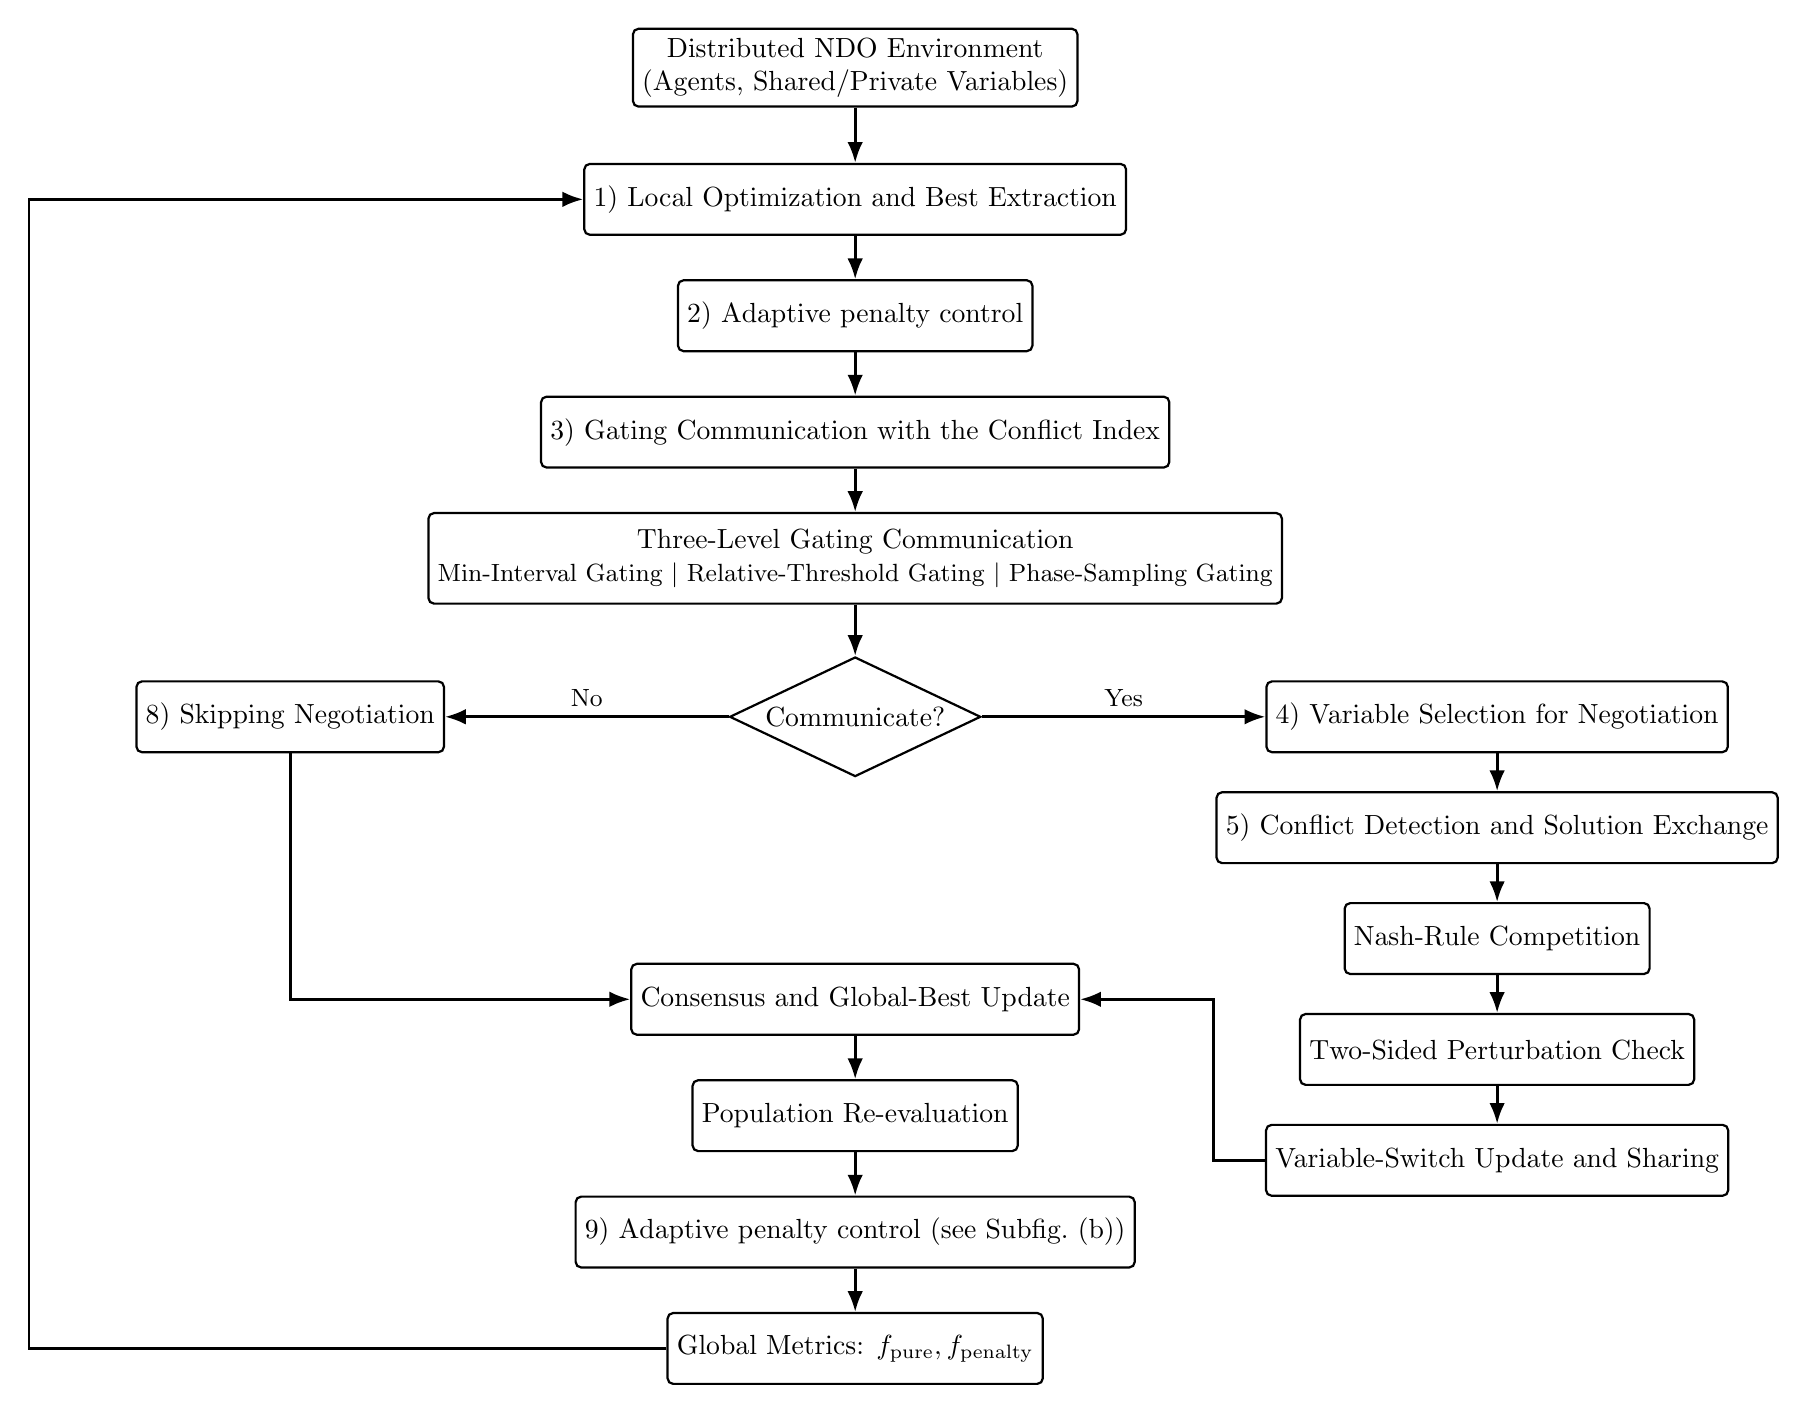
\begin{tikzpicture}[
  font=\normalsize,
  line/.style={-Latex, line width=1.0pt, draw=black},
  box/.style={rounded corners=2pt, draw=black, fill=white, line width=0.8pt, minimum width=3.6cm, minimum height=0.90cm, align=center},
  flow/.style={box},
  gate/.style={box, minimum width=4.1cm, minimum height=1.15cm},
  nego/.style={box, minimum width=3.7cm},
  skip/.style={box, minimum width=3.2cm},
  decision/.style={diamond, draw=black, fill=white, line width=0.8pt, aspect=2.1, inner sep=1.8pt, align=center}
]
\node[flow] (env) at (0,5.7) {Distributed NDO Environment\\(Agents, Shared/Private Variables)};
\node[flow, below=0.70cm of env] (opt) {1) Local Optimization and Best Extraction};
\node[flow, below=0.55cm of opt] (best) {2) Adaptive penalty control};
\node[flow, below=0.55cm of best] (conf) {3) Gating Communication with the Conflict Index};
\node[gate, below=0.55cm of conf] (gating) {Three-Level Gating Communication \\{\small Min-Interval Gating $\mid$ Relative-Threshold Gating $\mid$ Phase-Sampling Gating}};
\node[decision, below=0.65cm of gating] (decide) {Communicate?};

\node[nego, right=3.6cm of decide] (sel) {4) Variable Selection for Negotiation};
\node[nego, below=0.48cm of sel] (ex) {5) Conflict Detection and Solution Exchange};
\node[nego, below=0.48cm of ex] (nash) {Nash-Rule Competition};
\node[nego, below=0.48cm of nash] (pert) {Two-Sided Perturbation Check};
\node[nego, below=0.48cm of pert] (vsw) {Variable-Switch Update and Sharing};
\node[skip, left=3.6cm of decide] (skp) {8) Skipping Negotiation};

\node[flow, below=2.35cm of decide] (cons) {Consensus and Global-Best Update};
\node[flow, below=0.55cm of cons] (reeval) {Population Re-evaluation};
\node[flow, below=0.55cm of reeval] (rlstep) {9) Adaptive penalty control (see Subfig.~(b))};
\node[flow, below=0.55cm of rlstep] (metrics) {Global Metrics: $f_{\mathrm{pure}}, f_{\mathrm{penalty}}$};

\draw[line] (env.south) -- (opt.north);
\draw[line] (opt.south) -- (best.north);
\draw[line] (best.south) -- (conf.north);
\draw[line] (conf.south) -- (gating.north);
\draw[line] (gating.south) -- (decide.north);

\draw[line] (decide.east) -- node[above, font=\small] {Yes} (sel.west);
\draw[line] (sel) -- (ex);
\draw[line] (ex) -- (nash);
\draw[line] (nash) -- (pert);
\draw[line] (pert) -- (vsw);
\draw[line] (vsw.west) -- ++(-0.65cm,0) |- (cons.east);

\draw[line] (decide.west) -- node[above, font=\small] {No} (skp.east);
\coordinate (skipDownTurn) at (skp.south |- cons.west);
\draw[line] (skp.south) -- (skipDownTurn) -- (cons.west);

\draw[line] (cons) -- (reeval);
\draw[line] (reeval) -- (rlstep);
\draw[line] (rlstep) -- (metrics);
\coordinate (feedbackLeftTop) at ([xshift=-1.35cm]skp.west|-opt.west);
\coordinate (feedbackLeftBottom) at ([xshift=-1.35cm]skp.west|-metrics.west);
\draw[line] (metrics.west) -- (feedbackLeftBottom) -- (feedbackLeftTop) -- (opt.west);
\end{tikzpicture}%
}
\caption{Main per-iteration pipeline aligned with the implementation order. The numbered steps correspond to the subsection titles in Section~\protect\ref{sec:method}.}
\label{fig:rl_macpo_main}
\end{subfigure}
% --- END PATCHED FIGURE (a) ---
\hfill
% Subfigure (b)
\begin{subfigure}[t]{0.30\textwidth}
  \centering
  \resizebox{\linewidth}{!}{%
  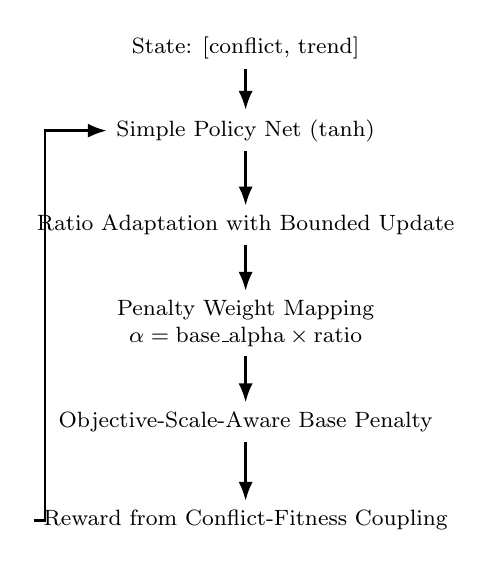
\begin{tikzpicture}[
    font=\footnotesize,
    txt/.style={align=center},
    flow/.style={-Latex, line width=0.85pt, draw=black},
    loopline/.style={-Latex, line width=0.85pt, draw=black}
  ]
  
  % compact text nodes
  \node[txt] (state)   at (0,5.2) {State: [conflict, trend]};
  \node[txt] (policy)  at (0,4.15) {Simple Policy Net ($\tanh$)};
  \node[txt] (ratio)   at (0,2.95) {Ratio Adaptation with Bounded Update};
  \node[txt] (map)     at (0,1.70) {Penalty Weight Mapping\\$\alpha = \mathrm{base\_alpha}\times \mathrm{ratio}$};
  \node[txt] (base)    at (0,0.45) {Objective-Scale-Aware Base Penalty};
  \node[txt] (reward)  at (0,-0.80) {Reward from Conflict-Fitness Coupling};
  
  % vertical arrows
  \draw[flow] (state.south)  -- (policy.north);
  \draw[flow] (policy.south) -- (ratio.north);
  \draw[flow] (ratio.south)  -- (map.north);
  \draw[flow] (map.south)    -- (base.north);
  \draw[flow] (base.south)   -- (reward.north);
  
  % left feedback loop
  \coordinate (leftA) at (-2.55,-0.80);
  \coordinate (leftB) at (-2.55,4.15);
  \draw[loopline] (reward.west) -- (leftA) -- (leftB) -- (policy.west);
  
  \end{tikzpicture}%
  }
  \caption{Adaptive penalty-control loop (RL default).}
  \label{fig:rl_macpo_rl}
\end{subfigure}

\caption{Overview of RL-MACPO. Subfigure (a) shows the main optimization and negotiation pipeline; Subfigure (b) details the adaptive penalty-control step (RL default) after re-evaluation.}
\label{fig:rl_macpo_architecture}
\end{figure*}


\paragraph{Pipeline reading guide.} Reading Fig.~\ref{fig:rl_macpo_architecture}(a) from top to bottom, each agent first evolves its local population under the current penalty, then evaluates whether communication is warranted from the logged conflict proxy. If the gate opens, neighbors exchange and compete on a subset of shared dimensions; otherwise the iteration skips negotiation and only refreshes the consensus reference. After population re-evaluation, the penalty module updates $\alpha_i$ for the next outer loop through the shared interface in Section~\ref{sec:penalty_interface}. Subfigure~(b) details the optional RL default for that penalty update; it is auxiliary to the communication gate in Subfigure~(a).

\subsection{Gating Communication with the Conflict Index}\label{sec:gating}
Conflict gating decides whether to open communication before paying the cost of neighbor negotiation. The gate uses a black-box conflict proxy $\mathrm{CI}_i^t$ to estimate whether another negotiation round is likely to improve shared consistency enough to justify its cost. A three-level rule (minimum interval, relative threshold with fail-safe, phase sampling) implements selective communication rather than a penalty update:
\begin{equation}
g_i^t=\mathbf{1}\left[\mathcal{C}_{\mathrm{int}}^t\land\bigl((\mathcal{C}_{\mathrm{rel}}^t\land \mathcal{C}_{\mathrm{phase}}^t)\lor \mathcal{C}_{\mathrm{fs}}^t\bigr)\right]
\label{eq:local_gate}
\end{equation}
Here $g_i^t=1$ means that agent $i$ requests communication at outer loop $t$. The interval condition $\mathcal{C}_{\mathrm{int}}^t$ prevents back-to-back negotiations that would add cost without fresh conflict information. The relative condition $\mathcal{C}_{\mathrm{rel}}^t:\ \mathrm{CI}_i^t > \lambda\,\hat{\mu}_{\mathrm{CI},i}^t$ opens the gate only when current conflict exceeds its recent EMA baseline $\hat{\mu}_{\mathrm{CI},i}^t$ by factor $\lambda$. The phase condition $\mathcal{C}_{\mathrm{phase}}^t:\ u_i^t < p_{\mathrm{phase}}^t$ with $u_i^t\sim\mathcal{U}(0,1)$ randomly thins communication according to search phase without per-function schedules. The fail-safe condition $\mathcal{C}_{\mathrm{fs}}^t:\ t-t_{\mathrm{last\_comm}}\ge K$ forces communication after $K$ silent outer loops so consensus references do not freeze; when $\mathcal{C}_{\mathrm{fs}}^t$ holds, phase sampling is bypassed. Thus Eq.~\eqref{eq:local_gate} is a three-layer \emph{communication trigger}, not a rule for updating $\alpha_i$.

A crucial implementation point is that $\mathrm{CI}_i^t$ is a black-box proxy motivated by the gradient-based conflict index in \cite{ref_macpo}, not a direct gradient estimate. For each overlapping dimension $d$, the proxy aggregates normalized discrepancies between the local best and the consensus reference; $\mathrm{CI}_i^t$ is their mean over the active overlap set.

\paragraph{Design rationale.} Layer~1 (minimum interval) prevents back-to-back negotiations that add cost without fresh conflict information. Layer~2 (relative threshold) opens communication only when local conflict exceeds its recent baseline, filtering weak or stale inconsistency. Fail-safe $K$ forces communication when the silent interval reaches $K$ outer loops, bypassing phase sampling so consensus references do not freeze. Layer~3 (phase sampling) modulates communication density on the relative-threshold path across search stages without per-function schedules. Together, these layers implement selective communication---the primary lever for the substantial communication reductions reported in Section~\ref{sec:exp_q2}.

In the parallel implementation, local requests are aggregated by
\begin{equation}
g_{\mathrm{global}}^t=\max_i g_i^t
\label{eq:global_gate}
\end{equation}
where $g_{\mathrm{global}}^t=1$ if \emph{any} agent requests communication at loop $t$. Eq.~\eqref{eq:global_gate} ensures that a neighborhood enters the negotiation branch whenever at least one agent observes conflict worth coordinating; otherwise all agents follow the skip-negotiation branch and refresh consensus references only.

Algorithm~\ref{alg:ci_gating} summarizes the gating procedure. Gate variants (always-on, fixed absolute threshold, relative threshold, relative threshold with fail-safe) are evaluated empirically in Section~\ref{sec:gate_validation}.

\begin{algorithm}[t]
  \footnotesize
  \caption{Conflict-Gated Communication with Phase Sampling (Abstract)}
  \label{alg:ci_gating}
  \begin{algorithmic}[1]
  \Require Local-best $x_i^\star$, consensus reference $x_{i,\mathrm{con}}$, overlap set $\Theta_i$, communication records
  \Ensure Global gate $g_{\mathrm{global}}^t$, communication branch selection
  \For{each optimization iteration $t$}
    \State Compute local conflict index $\mathrm{CI}_i^t$ on $\Theta_i$
    \State Update EMA statistic $\hat{\mu}_{\mathrm{CI},i}^t$ and the last-communication record
    \State Check interval constraint $\mathcal{C}_{\mathrm{int}}^t$ from communication cooldown
    \State Check relative threshold $\mathcal{C}_{\mathrm{rel}}^t: \mathrm{CI}_i^t > \lambda\hat{\mu}_{\mathrm{CI},i}^t$
    \State Check fail-safe $\mathcal{C}_{\mathrm{fs}}^t: t-t_{\mathrm{last\_comm}}\ge K$
    \State Draw phase sample $u_i^t\sim\mathcal{U}(0,1)$ and check $\mathcal{C}_{\mathrm{phase}}^t: u_i^t<p_{\mathrm{phase}}^t$
    \State Local gate:
    \Statex \hspace{1.5em}$g_i^t\gets \mathbf{1}\left[\mathcal{C}_{\mathrm{int}}^t\land((\mathcal{C}_{\mathrm{rel}}^t\land \mathcal{C}_{\mathrm{phase}}^t)\lor \mathcal{C}_{\mathrm{fs}}^t)\right]$
    \State Global reduction $g_{\mathrm{global}}^t\gets \max_i g_i^t$
    \If{$g_{\mathrm{global}}^t=0$}
      \State Follow skip-negotiation branch and keep local evolution only
      \State Refresh consensus reference from local-best maintenance rule
    \Else
      \State Enter negotiation branch for active neighbor pairs
      \State Execute exchange, competition, consistency check, and sharing in sequence
    \EndIf
    \State Update communication counters, interval timers, and threshold state
  \EndFor
  \State \Return Communication decisions and branch traces
  \end{algorithmic}
\end{algorithm}

\subsection{Variable Selection for Negotiation}\label{sec:selection}
Once communication is granted, variable selection decides \emph{which} shared dimensions enter negotiation: dimensions are ranked by an importance score $q_d^t$ and only a phase-dependent subset is processed (Fig.~\ref{fig:smart_selection_png}).

\begin{figure}[!t]
\centering
\resizebox{\linewidth}{!}{%
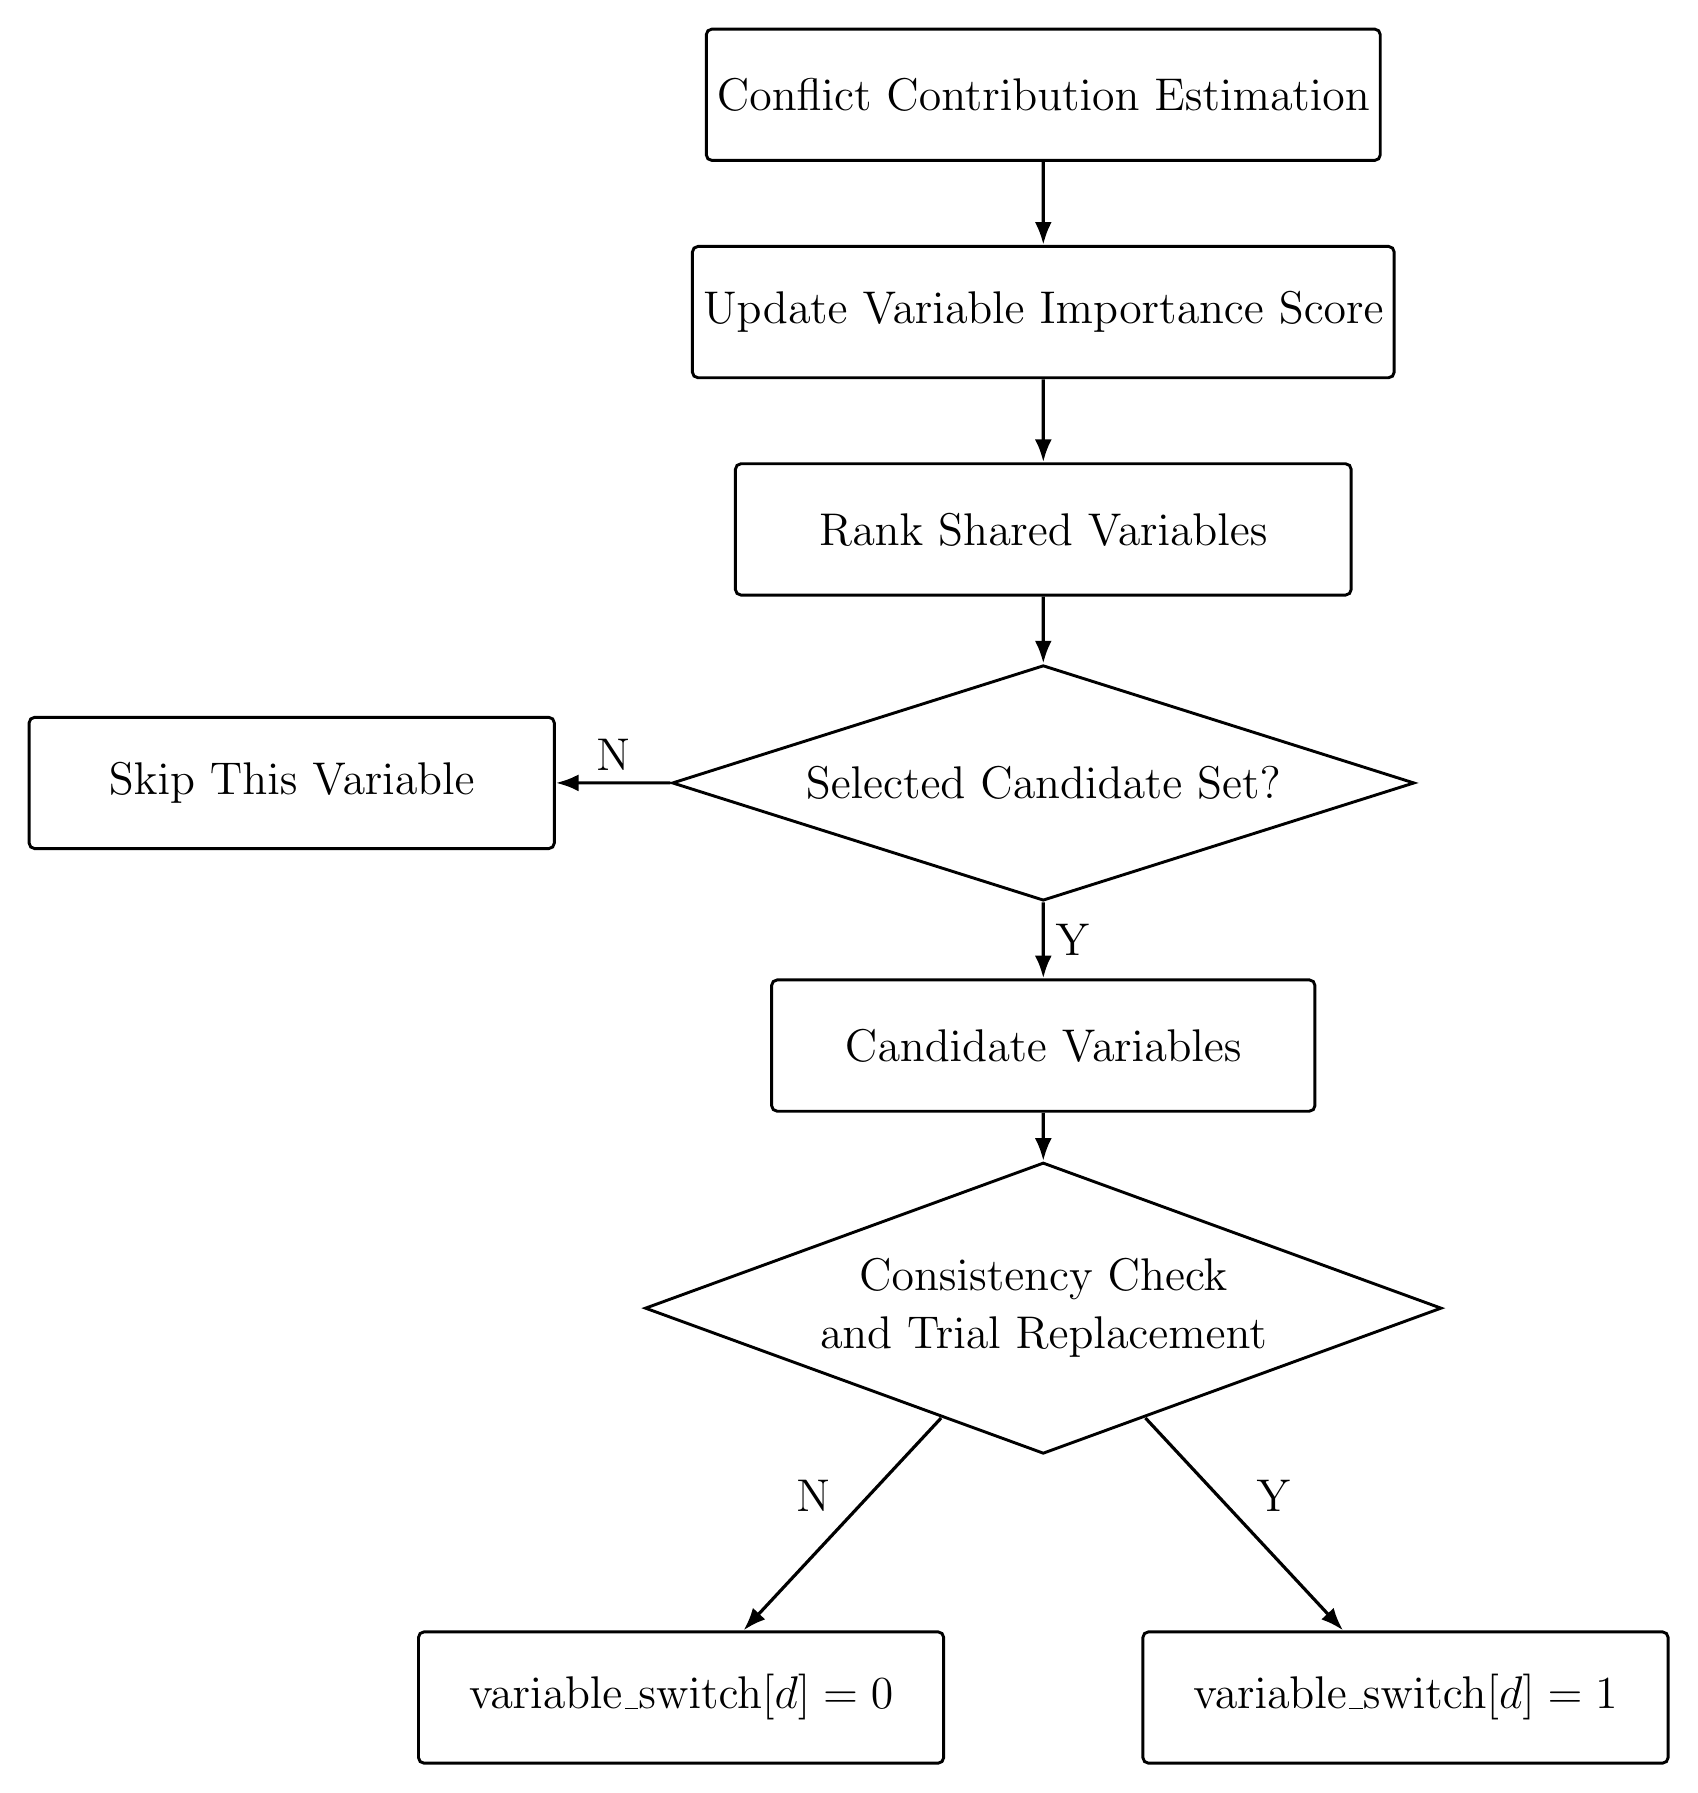
\begin{tikzpicture}[
  font=\Large, scale=1.15, every node/.style={transform shape},
  selbox/.style={draw=black, rounded corners=2pt, line width=1.05pt, minimum width=6.8cm, minimum height=1.45cm, align=center, fill=white},
  seldiamond/.style={diamond, draw=black, line width=1.05pt, aspect=2.7, inner sep=3.2pt, align=center, fill=white},
  selarrow/.style={-Latex, line width=1.15pt, draw=black}
]

% top vertical chain
\node[selbox] (conflict) at (0,10.2) {Conflict Contribution Estimation};
\node[selbox] (score)    at (0,7.8)  {Update Variable Importance Score};
\node[selbox] (rank)     at (0,5.4)  {Rank Shared Variables};
\node[seldiamond, minimum width=8.2cm, minimum height=2.35cm] (cand) at (0,2.6) {Selected Candidate Set?};

% left and right branches from first decision
% left and right branches from first decision
\node[selbox, minimum width=5.8cm] (skip) at (-8.3,2.6) {Skip This Variable};
\node[selbox, minimum width=6.0cm] (vars) at (0,-0.3) {Candidate Variables};

% second decision and final outputs
\node[seldiamond, minimum width=8.8cm, minimum height=2.55cm] (check) at (0,-3.2) {Consistency Check\\and Trial Replacement};
\node[selbox, minimum width=5.8cm] (off) at (-4.0,-7.5) {$\mathrm{variable\_switch}[d]=0$};
\node[selbox, minimum width=5.8cm] (on)  at (4.0,-7.5) {$\mathrm{variable\_switch}[d]=1$};

% main arrows
\draw[selarrow] (conflict) -- (score);
\draw[selarrow] (score) -- (rank);
\draw[selarrow] (rank) -- (cand);
\draw[selarrow] (cand) -- node[above, font=\Large] {N} (skip);
\draw[selarrow] (cand) -- node[right, font=\Large] {Y} (vars);
\draw[selarrow] (vars) -- (check);
\draw[selarrow] (check) -- node[above left, font=\Large] {N} (off);
\draw[selarrow] (check) -- node[above right, font=\Large] {Y} (on);

\end{tikzpicture}%
}
\caption{Variable Selection for Negotiation and Switch Control (Abstract)}
\label{fig:smart_selection_png}
\end{figure}

This can be viewed as importance sampling over shared variables---negotiation effort concentrates on dimensions whose historical conflict contribution is largest. The \emph{NoSelection} ablation disables this filter.

The goal of variable selection is to prioritize high-impact dimensions. For each shared variable $d$, the importance score evolves as
\begin{equation}
q_d^{t+1}=\gamma q_d^t+(1-\gamma)\,\xi_d^t,
\label{eq:importance_score}
\end{equation}
where $q_d^t$ accumulates historical evidence that dimension $d$ contributes to cross-agent conflict, $\xi_d^t$ is the current conflict-and-negotiation effectiveness signal for $d$, and $\gamma\in(0,1)$ controls smoothing. Eq.~\eqref{eq:importance_score} turns per-dimension conflict history into a ranking key used only \emph{after} the gate opens; it does not replace Eq.~\eqref{eq:local_gate}.

On the candidate dimension set $\Theta_i$, dimensions are ranked by $q_d^t$ and a subset $\Omega_i^t\subseteq\Theta_i$ enters negotiation. Skipping low-$q_d$ dimensions avoids perturbing shared variables that are already near consensus.

\paragraph{Role in communication quality.} Skipping low-$q_d$ dimensions avoids negotiation perturbations on shared variables that are already near consensus. Combined with gating, this shifts coordination from quantity (how often agents communicate) to quality (which rounds and dimensions are worth updating). Section~\ref{sec:q3_modules} ablates gating depth and related knobs; selection is part of the default \emph{Full} stack throughout the main benchmark.

\subsection{Conflict Detection and Solution Exchange}
When communication is active, neighbors exchange local-best candidates and apply Nash-style bilateral comparison followed by two-sided perturbation checking (Algorithm~\ref{alg:negotiation_consistency}).

\begin{algorithm}[t]
  \footnotesize
  \caption{Negotiation with Two-Sided Consistency Check (Abstract)}
  \label{alg:negotiation_consistency}
  \begin{algorithmic}[1]
  \Require Neighbor pair $(i,j)$, local-best candidates $x_i^\star,x_j^\star$, shared set $L_{i,j}$, variable switch $\mathrm{switch}[\cdot]$
  \Ensure Updated shared variables, consensus reference, and negotiation-success flag
  \State Exchange $x_i^\star$ and $x_j^\star$ between neighbors
  \State Initialize negotiation-success flag as false
  \For{each shared dimension $d\in L_{i,j}$}
    \If{$\mathrm{switch}[d]=0$}
      \State \textbf{continue}
    \EndIf
    \State Build local trial and cross trial for dimension $d$
    \State Evaluate utilities $u_{\mathrm{self}}(d)$, $u_{\mathrm{cross}}(d)$,
    \Statex \hspace{1.5em}$u_{\mathrm{cross,self}}(d)$, $u_{\mathrm{self,cross}}(d)$
    \If{$u_{\mathrm{self}}(d)+u_{\mathrm{cross,self}}(d) > u_{\mathrm{cross}}(d)+u_{\mathrm{self,cross}}(d)$}
      \State Select neighbor value for $d$
    \Else
      \State Keep local value for $d$
    \EndIf
    \State Perform two-sided perturbation around selected value on $d$
    \State Obtain responses $(\delta_i^+,\delta_i^-)$ and $(\delta_j^+,\delta_j^-)$
    \If{$(\delta_i^+\delta_j^+>0)\land(\delta_i^-\delta_j^->0)$}
      \State $\mathrm{switch}[d]\gets 0$
    \Else
      \State Keep $\mathrm{switch}[d]$ active for future renegotiation
    \EndIf
    \State If accepted by sharing rule, write updated $d$ into consensus reference
    \State Update negotiation-success flag when at least one dimension changes
  \EndFor
  \State Re-evaluate local population under new consensus reference
  \State \Return Consensus reference, $\mathrm{switch}[\cdot]$, negotiation-success flag
  \end{algorithmic}
\end{algorithm}

\subsection{Adaptive Penalty Control Interface}\label{sec:penalty_interface}
The penalty module exposes a common interface---conflict signals in, bounded penalty ratio out---implemented by RL (default), EMA smoothing, or fixed phase schedules (Table~\ref{tab:penalty_controller_f3_f5}). All implementations share the same ratio mapping; they differ only in how $\rho_i^{t+1}$ is updated. This module stabilizes local search under Eq.~\eqref{eq:macpo_local_objective}; it is not the communication gate in Eq.~\eqref{eq:local_gate}.

The conflict term fed to local search and to the controller is
\begin{equation}
c_i(x)=\sum_{d\in\Theta_i}\frac{|x^d-x_{i,\mathrm{con}}^d|}{u_d-l_d}
\label{eq:conflict_term}
\end{equation}
where $x_{i,\mathrm{con}}^d$ is the consensus reference for dimension $d$, and $u_d-l_d$ normalizes by the box bounds. Eq.~\eqref{eq:conflict_term} measures how far agent $i$'s candidate deviates from the neighborhood reference on each active dimension.

Under the RL default, the controller observes
\begin{equation}
s_i^t=[c_i^t,\ \Delta c_i^t],\qquad \Delta c_i^t=c_i^t-c_i^{t-1}
\label{eq:rl_state}
\end{equation}
where $s_i^t$ summarizes current conflict level and its short-term trend, and produces a bounded action
\begin{equation}
a_i^t=\pi_\theta(s_i^t),\qquad a_i^t\in(-1,1)
\label{eq:rl_action}
\end{equation}
with $\pi_\theta$ a lightweight policy network. The action adjusts a penalty ratio rather than opening communication:
\begin{subequations}
\begin{align}
\rho_i^{t+1}&=\Pi_{[\rho_{\min},\rho_{\max}]}
\left(\rho_i^t+\eta_a a_i^t\right),
\label{eq:rho_update}\\
\alpha_i^{t+1}&=\bar{\alpha}_i^{t+1}\rho_i^{t+1}.
\label{eq:alpha_mapping}
\end{align}
\end{subequations}
Here $\Pi$ projects the ratio into $[\rho_{\min},\rho_{\max}]$, $\bar{\alpha}_i$ is an objective-scale baseline penalty, and $\rho_i$ provides online adaptation of $\alpha_i$ in Eq.~\eqref{eq:macpo_local_objective}. Eqs.~\eqref{eq:rho_update}--\eqref{eq:alpha_mapping} therefore implement \emph{penalty strength control}, orthogonal to the gate in Eq.~\eqref{eq:local_gate}.

The RL default learns $\pi_\theta$ from a bounded reward that couples conflict reduction with pure-objective improvement:
\begin{equation}
r_i^t=\psi\left(-\Delta c_{i,\mathrm{rate}}^t\cdot \Delta f_{i,\mathrm{pure,rate}}^t\right)
\label{eq:rl_reward}
\end{equation}
where $\psi(\cdot)$ is an odd squashing map, $\Delta c_{i,\mathrm{rate}}^t$ is the relative change in conflict, and $\Delta f_{i,\mathrm{pure,rate}}^t$ is the relative change in logged pure objective. Eq.~\eqref{eq:rl_reward} encourages penalty updates that reduce conflict without harming pure fitness. EMA and fixed schedules plug into the same $\rho$--$\alpha$ mapping without policy learning. Algorithm~\ref{alg:rl_penalty_update} summarizes the RL default; heuristic controllers replace the policy/replay steps with their own $\rho$-update rules.

\begin{algorithm}[t]
  \footnotesize
  \caption{Adaptive Penalty Control with RL Default (Abstract)}
  \label{alg:rl_penalty_update}
  \begin{algorithmic}[1]
  \Require Conflict and baseline-penalty streams, policy $\pi_{\theta_i}$, replay buffer $\mathcal{B}_i$
  \Ensure Updated $\{\rho_i^t,\alpha_i^t,\theta_i\}$
  \For{each optimization iteration $t$}
    \State Form $s_i^t=[c_i^t,\Delta c_i^t]$ from shared-variable conflict (Eqs.~\eqref{eq:conflict_term}--\eqref{eq:rl_state})
    \State Infer $a_i^t=\pi_{\theta_i}(s_i^t)$ and map to $\rho_i^{t+1},\alpha_i^{t+1}$ (Eqs.~\eqref{eq:rho_update}--\eqref{eq:alpha_mapping})
    \State Optimize locally with $h_i(x)=f_i(x)+\alpha_i^{t+1}c_i(x)$; compute $r_i^t$ (Eq.~\eqref{eq:rl_reward})
    \State Append $(s_i^t,a_i^t,r_i^t)$ to $\mathcal{B}_i$ and update $\theta_i$ by prioritized replay when triggered
  \EndFor
  \end{algorithmic}
\end{algorithm}

\section{Experimental Setup and Results}\label{sec:experiments}
\subsection{Experimental Setup}
\paragraph{Benchmark.} We use the MACPO NDO suite F1--F18 \cite{ref_macpo} under the \emph{Full} RL-MACPO configuration unless an ablation caption states otherwise. Dispatch and IEEE cases are in Section~\ref{sec:applications}. Table~\ref{tab:benchmark_f1f6} lists the primary small-scale chain family (20 agents, $D{=}905$). Homogeneous instances F1--F3 share one base landscape per agent. Heterogeneous instances F4--F6 mix elliptic, Schwefel, and Rosenbrock segments. Theory CI in the table is the average conflict index from \cite{ref_macpo}. RL-MACPO uses a black-box conflict proxy in the same role for gating. By theory CI, F3 and F5 are high-conflict (0.846 and 0.497), F2 and F4 are low-conflict (0.049 and 0.051), and F1 and F6 are mid-range (0.228 and 0.268).

\begin{table}[!t]
\centering
\small
\caption{MACPO small-scale benchmark family F1--F6 (20-agent chain, $D{=}905$). F1--F3 are homogeneous; F4--F6 are heterogeneous \cite{ref_macpo}.}
\label{tab:benchmark_f1f6}
\begin{tabular}{@{}lll@{}}
\toprule
\textbf{Func.} & \textbf{Composition} & \textbf{Theory CI} \\
\midrule
\multicolumn{3}{@{}l}{\textit{Homogeneous}} \\
F1 & Elliptic & 0.228 \\
F2 & Schwefel & 0.049 \\
F3 & Rosenbrock & 0.846 \\
\addlinespace[0.15em]
\multicolumn{3}{@{}l}{\textit{Heterogeneous}} \\
F4 & Elliptic--Schwefel & 0.051 \\
F5 & Elliptic--Rosenbrock & 0.497 \\
F6 & Schwefel--Rosenbrock & 0.268 \\
\bottomrule
\end{tabular}
\end{table}

\paragraph{Benchmark family (Table~\ref{tab:benchmark_f1f6}).}
F1--F6 follow the MACPO NDO benchmark \cite{ref_macpo} on a 20-agent chain with $D{=}905$. \emph{Composition} names the constituent base functions. \emph{Theory CI} is the average conflict index from \cite{ref_macpo}. RL-MACPO uses an implementation conflict proxy in the same role for gating, not the gradient estimate directly. F7--F18 extend agent count and topology as in \cite{ref_macpo}.

\paragraph{Evaluation protocol.} MACPO and RL-MACPO share paired seeds, the MACPO evaluation-budget cap, and embedded optimizers LLSO \cite{ref_llso} (primary) and CSO \cite{ref_cso} (secondary). End-of-run evaluation counts differ by at most a few percent (Table~\ref{tab:comm_rate_f1_f18}). Wall-clock overhead is reported separately in Table~\ref{tab:wall_time_f1_f18} within Section~\ref{sec:exp_q1} and is not a primary endpoint.

\paragraph{Notation and statistics.} $F(\mathbf{X})$ denotes the global objective in Eq.~\eqref{eq:global_objective}. Logged $f_{\mathrm{pure}}$ is the pure objective sum without penalty terms. Logged $f_{\mathrm{penalty}}$ includes conflict penalties. Lower is better unless a caption states otherwise. Main tables report mean, median, standard deviation, and win/tie/loss over \textbf{25 independent runs}. RL-MACPO vs.\ MACPO uses paired Wilcoxon signed-rank tests (LLSO) or Mann--Whitney U tests (CSO) at the 0.05 significance level \cite{ref_macpo}. Boldface marks the better mean within each MACPO vs.\ RL-MACPO pair.

\subsection{Experimental Roadmap}\label{sec:exp_roadmap}

\begin{figure}[!t]
\centering
\resizebox{\columnwidth}{!}{%
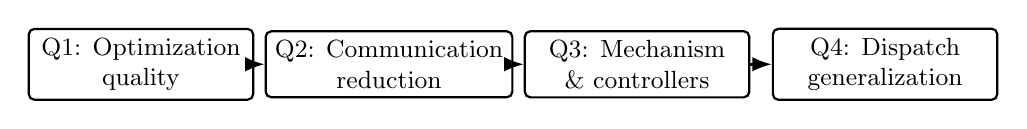
\begin{tikzpicture}[
  font=\small,
  box/.style={draw, rounded corners=2pt, line width=0.8pt, minimum width=2.85cm, minimum height=0.72cm, align=center, fill=white},
  arr/.style={-Latex, line width=0.9pt, draw=black}
]
\node[box] (q1) at (0,0) {Q1: Optimization\\quality};
\node[box] (q2) at (3.15,0) {Q2: Communication\\reduction};
\node[box] (q3) at (6.3,0) {Q3: Mechanism\\ \& controllers};
\node[box] (q4) at (9.45,0) {Q4: Dispatch\\generalization};
\draw[arr] (q1.east) -- (q2.west);
\draw[arr] (q2.east) -- (q3.west);
\draw[arr] (q3.east) -- (q4.west);
\end{tikzpicture}%
}
\caption{Experimental roadmap (left to right). Details for each block are in the text below.}
\label{fig:exp_roadmap}
\end{figure}


The evaluation is organized around four questions tied to the communication-efficiency goal of Section~\ref{sec:intro}. Fig.~\ref{fig:exp_roadmap} shows the reading order; the four blocks below state what each question tests and where the evidence appears.

\paragraph{Q1 (Optimization quality).}
Does RL-MACPO match or improve final fitness under the \emph{same} evaluation budget as MACPO? We compare paired 25-run batches on F1--F18 with LLSO (primary) and CSO (secondary), reporting mean, median, standard deviation, and significance (Tables~\ref{tab:macpo_style_all} and~\ref{tab:macpo_rl_mean_f1_f18}; convergence curves in Fig.~\ref{fig:fes_f1_f6_panel}).

\paragraph{Q2 (Communication reduction).}
Can conflict-gated communication cut negotiation rate without sacrificing Q1 fitness? We report outer-loop trigger rates, evaluation-budget parity, gate-variant diagnostics, and a communication--fitness trade-off (Tables~\ref{tab:comm_rate_f1_f18} and~\ref{tab:gate_cost_stats}; Fig.~\ref{fig:comm_fitness_pareto}).

\paragraph{Q3 (Mechanisms and controllers).}
Which modules matter, and is RL necessary once gating is fixed? Section~\ref{sec:q3_penalty} compares RL, EMA, and fixed penalty schedules on F3/F5 under identical gating; Section~\ref{sec:q3_modules} ablates gating layers, variable selection, phase sampling, and $\eta$ strategies (Table~\ref{tab:penalty_controller_f3_f5}, Fig.~\ref{fig:gating_ablation}, Tables~\ref{tab:deeprl} and~\ref{tab:phase_eta}).

\paragraph{Q4 (Dispatch generalization).}
Do benchmark savings transfer to MACPO-style dispatch simulators and IEEE transmission-network pilots? Section~\ref{sec:applications} reports paired communication rate and pure-objective change on application cases and IEEE~30/57/118 (Tables~\ref{tab:application_cases} and~\ref{tab:ieee_power_cases}).

\subsection{Question 1: Does RL-MACPO Preserve Optimization Quality?}\label{sec:exp_q1}
We compare paired 25-run batches on F1--F18 under the same evaluation budget.

\begin{table*}[!t]
\centering
\tiny
\setlength{\tabcolsep}{1.8pt}
\renewcommand{\arraystretch}{1.00}
\caption{Final global objective $F$ (Eq.~\protect\eqref{eq:global_objective}) on F1--F6: mean, median, standard deviation, and $p$-value over 25 independent runs, for LLSO (left five columns) and CSO (right five columns). \textbf{MACPO} and \textbf{RL-MACPO} use logged \texttt{f\_pure} (last row per run) from archived trajectories. \textbf{GFPDO$^{\dagger}$}: 25-run batch under the MACPO GFPDO executable (same evaluation budget); \textbf{DPSO$^{\dagger}$}: 25-run batch under the MACPO DPSO executable (same evaluation budget). No significance tests for external columns. Tests for RL-MACPO vs.\ MACPO only: paired Wilcoxon signed-rank (LLSO), Mann--Whitney U (CSO). * RL-MACPO better; \# worse ($p<0.05$). Shaded cells: better mean in each MACPO vs.\ RL-MACPO pair.}
\label{tab:macpo_style_all}
\resizebox{\textwidth}{!}{%
\begin{tabular}{llccccc|ccccc}
\toprule
\multirow{2}{*}{\makecell[c]{\textbf{Bench.}}} & \multirow{2}{*}{\textbf{Metric}} & \multicolumn{5}{c}{\textbf{LLSO}} & \multicolumn{5}{c}{\textbf{CSO}} \\
\cmidrule(lr){3-7}\cmidrule(lr){8-12}
& & \textbf{GFPDO$^{\dagger}$} & \textbf{DPSO$^{\dagger}$} & \textbf{MACPO} & \textbf{RL Only} & \textbf{RL-MACPO} & \textbf{GFPDO$^{\dagger}$} & \textbf{DPSO$^{\dagger}$} & \textbf{MACPO} & \textbf{RL Only} & \textbf{RL-MACPO} \\
\midrule
\multirow{4}{*}{F1}
& mean    & 2.90E+9 & 4.35E+10 & 1.98E+7 & 2.07E+7 & \bestval{6.43E+6} & 4.58E+10 & 8.84E+10 & 2.33E+7 & 2.02E+7 & \bestval{1.25E+7} \\
& median  & 2.90E+9 & 4.37E+10 & 2.00E+7 & 1.97E+7 & 6.48E+6 & 4.61E+10 & 8.82E+10 & 2.24E+7 & 2.00E+7 & 1.27E+7 \\
& std     & 1.63E+8 & 7.23E+9 & 1.71E+6 & 3.58E+6 & 3.52E+5 & 2.51E+9 & 4.27E+9 & 2.98E+6 & 1.34E+6 & 6.26E+5 \\
& p-value & --- & --- & - & 5.46e-01 & 2.98e-08* & --- & --- & - & 2.41e-05* & 6.90e-10* \\
\midrule
\multirow{4}{*}{F2}
& mean    & 2.29E+7 & 5.76E+9 & 5.05E+4 & 4.76E+4 & \bestval{3.32E+3} & 2.12E+10 & 1.55E+11 & 6.95E+4 & 6.43E+4 & \bestval{9.11E+3} \\
& median  & 2.33E+7 & 5.05E+9 & 4.83E+4 & 4.35E+4 & 3.33E+3 & 2.00E+10 & 1.49E+11 & 6.81E+4 & 6.38E+4 & 9.09E+3 \\
& std     & 1.99E+6 & 3.01E+9 & 6.23E+3 & 9.67E+3 & 1.33E+2 & 5.20E+9 & 4.84E+10 & 5.90E+3 & 6.98E+3 & 8.06E+2 \\
& p-value & --- & --- & - & 5.46e-01 & 2.98e-08* & --- & --- & - & 2.41e-05* & 7.07e-10* \\
\midrule
\multirow{4}{*}{F3}
& mean    & 6.00E+10 & 2.19E+11 & 4.03E+9 & 5.89E+9 & \bestval{6.35E+2} & 3.60E+11 & 6.08E+11 & 1.51E+9 & 2.66E+9 & \bestval{6.70E+2} \\
& median  & 5.93E+10 & 2.18E+11 & 4.05E+9 & 5.86E+9 & 6.32E+2 & 3.65E+11 & 6.00E+11 & 1.51E+9 & 2.60E+9 & 6.45E+2 \\
& std     & 2.85E+9 & 6.37E+9 & 4.79E+8 & 7.13E+8 & 3.12E+1 & 2.11E+10 & 3.64E+10 & 8.57E+7 & 2.64E+8 & 2.63E+2 \\
& p-value & --- & --- & - & 5.46e-01 & 2.98e-08* & --- & --- & - & 2.41e-05* & 6.98e-10* \\
\midrule
\multirow{4}{*}{F4}
& mean    & 7.92E+8 & 2.49E+10 & 3.17E+6 & 3.01E+6 & \bestval{2.58E+6} & 3.00E+10 & 6.35E+10 & 7.30E+6 & 6.98E+6 & \bestval{5.80E+6} \\
& median  & 7.90E+8 & 2.38E+10 & 3.14E+6 & 2.98E+6 & 2.61E+6 & 2.98E+10 & 6.14E+10 & 7.16E+6 & 6.90E+6 & 5.80E+6 \\
& std     & 6.11E+7 & 5.34E+9 & 3.59E+5 & 2.71E+5 & 1.29E+5 & 2.17E+9 & 6.59E+9 & 7.53E+5 & 9.53E+5 & 3.82E+5 \\
& p-value & --- & --- & - & 5.46e-01 & 8.94e-08* & --- & --- & - & 2.41e-05* & 1.82e-09* \\
\midrule
\multirow{4}{*}{F5}
& mean    & 2.27E+10 & 8.80E+10 & 1.97E+8 & 4.24E+8 & \bestval{3.50E+6} & 1.52E+11 & 1.98E+11 & 2.50E+7 & 4.98E+7 & \bestval{6.61E+6} \\
& median  & 2.27E+10 & 8.84E+10 & 1.98E+8 & 4.10E+8 & 3.52E+6 & 1.52E+11 & 1.98E+11 & 2.50E+7 & 4.75E+7 & 6.66E+6 \\
& std     & 1.87E+9 & 1.25E+10 & 3.91E+7 & 1.08E+8 & 1.40E+5 & 7.36E+9 & 2.28E+10 & 1.75E+6 & 1.31E+7 & 5.02E+5 \\
& p-value & --- & --- & - & 5.46e-01 & 2.98e-08* & --- & --- & - & 2.41e-05* & 7.07e-10* \\
\midrule
\multirow{4}{*}{F6}
& mean    & 2.75E+10 & 8.81E+10 & 1.62E+8 & 1.50E+8 & \bestval{2.47E+3} & 1.98E+11 & 3.98E+11 & 3.40E+6 & 4.29E+5 & \bestval{5.56E+3} \\
& median  & 2.75E+10 & 8.48E+10 & 5.04E+7 & 1.36E+8 & 2.47E+3 & 1.99E+11 & 3.96E+11 & 6.51E+5 & 3.73E+5 & 5.20E+3 \\
& std     & 2.26E+9 & 1.36E+10 & 2.20E+8 & 1.47E+8 & 1.02E+2 & 1.83E+10 & 6.25E+10 & 6.80E+6 & 1.87E+5 & 9.78E+2 \\
& p-value & --- & --- & - & 5.46e-01 & 2.98e-08* & --- & --- & - & 2.41e-05* & 7.08e-10* \\
\midrule
\multicolumn{2}{c}{w/t/l} & --- & --- & - & 1/3/2 & 6/0/0 & --- & --- & - & 3/1/2 & 6/0/0 \\
\bottomrule
\end{tabular}
}
\end{table*}


Table~\ref{tab:macpo_style_all} reports F1--F6 with mean, median, standard deviation, and significance for LLSO and CSO.

\begin{table*}[!t]
\centering
\scriptsize
\setlength{\tabcolsep}{2.5pt}
\renewcommand{\arraystretch}{0.88}
\caption{Budget-endpoint comparison on F7--F18 over 25 independent runs: MACPO vs.\ RL-MACPO under LLSO and CSO. \textbf{MACPO$^{\ddagger}$} reports mean $\pm$ sample std of archived endpoint $F$ (still penalized when overlap inconsistency remains). \textbf{RL-MACPO} reports mean $\pm$ sample std of terminal logged $f_{\mathrm{pure}}$, which equals $f_{\mathrm{penalty}}$ in all archived runs. The two columns use different endpoint definitions; large gaps on F9/F15 reflect MACPO failing to eliminate overlap inconsistency under static penalties. Lower is better; shaded cells mark the better mean within each pair. Last row: w/t/l.}
\label{tab:macpo_rl_mean_f1_f18}
\begin{minipage}[t]{0.49\textwidth}
\centering
\resizebox{\linewidth}{!}{%
\begin{minipage}{\linewidth}
\centering
\textbf{(a) F7--F12}\\[0.3em]
\begin{tabular}{@{}lcccc@{}}
\toprule
 & \multicolumn{2}{c}{\textbf{LLSO}} & \multicolumn{2}{c}{\textbf{CSO}} \\
\cmidrule(lr){2-3}\cmidrule(lr){4-5}
\textbf{Func.} & \textbf{MACPO} & \textbf{RL-MACPO} & \textbf{MACPO} & \textbf{RL-MACPO} \\
\midrule
F7 & \makecell{2.30E+9\\$\pm$2.05E+8} & \beststat{1.44E+7}{4.56E+5} & \makecell{3.29E+9\\$\pm$1.61E+8} & \beststat{4.58E+7}{1.40E+6} \\
F8 & \makecell{1.27E+7\\$\pm$5.49E+5} & \beststat{6.19E+4}{4.11E+3} & \makecell{2.77E+7\\$\pm$1.45E+6} & \beststat{4.20E+5}{1.96E+4} \\
F9 & \makecell{3.05E+11\\$\pm$1.17E+10} & \beststat{1.01E+3}{2.48E+2} & \makecell{2.40E+11\\$\pm$8.64E+9} & \beststat{1.04E+3}{2.12E+2} \\
F10 & \makecell{1.10E+9\\$\pm$7.57E+7} & \beststat{7.10E+6}{3.41E+5} & \makecell{1.97E+9\\$\pm$1.59E+8} & \beststat{2.39E+7}{9.98E+5} \\
F11 & \makecell{5.43E+10\\$\pm$3.84E+9} & \beststat{7.03E+6}{2.48E+5} & \makecell{4.90E+10\\$\pm$3.69E+9} & \beststat{2.34E+7}{8.36E+5} \\
F12 & \makecell{5.39E+10\\$\pm$6.20E+9} & \beststat{2.79E+4}{2.56E+3} & \makecell{5.33E+10\\$\pm$6.02E+9} & \beststat{2.39E+5}{1.64E+5} \\
\bottomrule
\end{tabular}
\end{minipage}%
}
\end{minipage}\hfill
\begin{minipage}[t]{0.49\textwidth}
\centering
\resizebox{\linewidth}{!}{%
\begin{minipage}{\linewidth}
\centering
\textbf{(b) F13--F18}\label{tab:macpo_rl_mean_f1_f18_b}\\[0.3em]
\begin{tabular}{@{}lcccc@{}}
\toprule
 & \multicolumn{2}{c}{\textbf{LLSO}} & \multicolumn{2}{c}{\textbf{CSO}} \\
\cmidrule(lr){2-3}\cmidrule(lr){4-5}
\textbf{Func.} & \textbf{MACPO} & \textbf{RL-MACPO} & \textbf{MACPO} & \textbf{RL-MACPO} \\
\midrule
F13 & \makecell{6.96E+9\\$\pm$2.22E+8} & \beststat{2.91E+7}{6.73E+5} & \makecell{1.17E+10\\$\pm$2.75E+8} & \beststat{2.05E+8}{4.63E+6} \\
F14 & \makecell{6.20E+7\\$\pm$1.41E+6} & \beststat{5.20E+5}{1.94E+4} & \makecell{3.49E+8\\$\pm$2.33E+7} & \beststat{6.91E+6}{2.91E+5} \\
F15 & \makecell{1.24E+12\\$\pm$2.41E+10} & \beststat{8.41E+2}{1.89E+2} & \makecell{9.02E+11\\$\pm$1.51E+10} & \beststat{8.20E+2}{1.71E+2} \\
F16 & \makecell{2.93E+9\\$\pm$8.03E+7} & \beststat{1.50E+7}{4.70E+5} & \makecell{7.06E+9\\$\pm$2.92E+8} & \beststat{1.07E+8}{4.46E+6} \\
F17 & \makecell{2.17E+11\\$\pm$9.72E+9} & \beststat{1.38E+7}{4.13E+5} & \makecell{1.74E+11\\$\pm$9.28E+9} & \beststat{1.04E+8}{2.85E+6} \\
F18 & \makecell{2.28E+11\\$\pm$1.44E+10} & \beststat{2.61E+5}{1.12E+4} & \makecell{2.01E+11\\$\pm$1.51E+10} & \beststat{3.27E+6}{1.32E+5} \\
\bottomrule
\end{tabular}
\end{minipage}%
}
\end{minipage}
\end{table*} In this table, * marks RL-MACPO better and \# marks worse. The table also lists \emph{RL Only} (adaptive penalty without gating) for reference; GFPDO$^{\dagger}$/DPSO$^{\dagger}$ columns follow the MACPO paper layout \cite{ref_macpo} without significance tests.

Table~\ref{tab:macpo_rl_mean_f1_f18} extends the same comparison to F7--F18 (panels (a)--(b)).

\begin{table*}[!t]
\centering
\tiny
\setlength{\tabcolsep}{2.8pt}
\caption{Indicative mean wall-clock time per run (\textbf{seconds}) on F1--F18, measured on our development hardware during the same 25-run batch as Table~\protect\ref{tab:macpo_rl_mean_f1_f18}; values are for qualitative overhead comparison only (RL policy inference and gating bookkeeping), not hardware-normalized benchmarks. The archived fitness trajectory logs used for Tables~\protect\ref{tab:macpo_style_all} and~\protect\ref{tab:macpo_rl_mean_f1_f18} do not uniformly record wall-clock timestamps; these entries were taken from end-of-run timing notes on the batch machine and are not automatically recomputable from the fitness log archive alone.}
\label{tab:wall_time_f1_f18}
\resizebox{\textwidth}{!}{%
\begin{tabular}{l*{18}{c}}
\toprule
\textbf{Setting} & F1 & F2 & F3 & F4 & F5 & F6 & F7 & F8 & F9 & F10 & F11 & F12 & F13 & F14 & F15 & F16 & F17 & F18 \\
\midrule
MACPO / LLSO & 14.43 & 13.87 & 8.56 & 14.30 & 13.34 & 12.92 & 156.29 & 148.05 & 114.41 & 149.51 & 148.21 & 164.68 & 1303.45 & 1316.65 & 1046.99 & 1378.96 & 1222.45 & 1768.14 \\
RL-MACPO / LLSO & 26.95 & 26.43 & 19.11 & 26.08 & 22.70 & 23.05 & 296.98 & 294.08 & 271.95 & 296.16 & 147.13 & 146.87 & 2540.74 & 2571.82 & 2288.38 & 2512.78 & 2374.17 & 2467.96 \\
\midrule
MACPO / CSO & 14.72 & 14.10 & 8.53 & 14.20 & 13.35 & 12.92 & 169.95 & 88.28 & 67.30 & 92.06 & 161.36 & 169.10 & 1477.39 & 738.38 & 618.22 & 755.67 & 1430.60 & 1445.48 \\
RL-MACPO / CSO & 29.07 & 27.83 & 21.08 & 27.48 & 24.39 & 24.30 & 351.61 & 413.60 & 288.47 & 343.87 & 329.01 & 302.33 & 2984.85 & 1528.16 & 1399.31 & 1549.00 & 1482.71 & 1452.14 \\
\bottomrule
\end{tabular}%
}
\end{table*}

On our development machine, RL-MACPO runs about twice as long as MACPO on F1--F6 (for example 27\,s vs.\ 14\,s on F1 under LLSO). Table~\ref{tab:wall_time_f1_f18} lists indicative wall-clock times for all functions. These numbers reflect RL policy inference and gating bookkeeping, not hardware-normalized benchmarks.

Figure~\ref{fig:fes_f1_f6_panel} shows paired best-so-far curves (one run per function; 25-run aggregates in Table~\ref{tab:macpo_style_all}).

\paragraph{Q1 analysis.} Gated RL-MACPO wins every F1--F6 and F7--F18 comparison at the same evaluation budget (w/t/l 6/0/0 and 12/0/0). The gain is largest on high-conflict Rosenbrock-related instances and on F9/F15, where always-on MACPO fails to restore shared-variable consistency under static penalties (Table~\ref{tab:macpo_rl_mean_f1_f18}). \emph{RL Only} without gating remains weaker on F3/F5 (Table~\ref{tab:macpo_style_all}), so the improvement requires conflict gating rather than adaptive penalty alone.

\subsection{Question 2: Does Conflict-Gated Communication Reduce Cost?}\label{sec:exp_q2}
MACPO negotiates on every outer loop. RL-MACPO triggers negotiation on only a fraction of outer loops while preserving or improving the Q1 fitness from Section~\ref{sec:exp_q1}. Table~\ref{tab:comm_rate_f1_f18} reports trigger rates on F1--F18. On F3--F6 the rate is 8.3\%, a 91.7\% reduction relative to always-on MACPO. On F1 it remains 20.8\%.

\begin{table}[!t]
\centering
\scriptsize
\setlength{\tabcolsep}{4pt}
\caption{Communication trigger rate on F1--F18 (LLSO, 25 paired runs). MACPO negotiates on every outer loop (baseline rate 100\%). End-of-run evaluation counts on F1--F6 are 145729 (MACPO) and 150348 (RL-MACPO), differing by about 3.2\%. Comm.\ drop is relative to always-on MACPO.}
\label{tab:comm_rate_f1_f18}
\begin{tabular}{@{}lcc@{}}
\toprule
\textbf{Func.} & \textbf{RL-MACPO comm.} & \textbf{Reduction} \\
\midrule
F1 & \textbf{20.8} & 79.2\% \\
F2 & \textbf{22.3{\scriptsize $\pm$4.1}} & 77.7\% \\
F3 & \textbf{8.3} & 91.7\% \\
F4 & \textbf{8.3} & 91.7\% \\
F5 & \textbf{8.3} & 91.7\% \\
F6 & \textbf{8.3} & 91.7\% \\
F7 & \textbf{8.0} & 92.0\% \\
F8 & \textbf{8.0} & 92.0\% \\
F9 & \textbf{8.0} & 92.0\% \\
F10 & \textbf{8.0} & 92.0\% \\
F11 & \textbf{8.0} & 92.0\% \\
F12 & \textbf{8.0} & 92.0\% \\
F13 & \textbf{7.7{\scriptsize $\pm$1.6}} & 92.3\% \\
F14 & \textbf{8.0} & 92.0\% \\
F15 & \textbf{8.0} & 92.0\% \\
F16 & \textbf{8.0} & 92.0\% \\
F17 & \textbf{8.0} & 92.0\% \\
F18 & \textbf{8.0} & 92.0\% \\
\bottomrule
\end{tabular}
\end{table}

\paragraph{Q2 analysis.} The relative-threshold gate suppresses negotiation when the logged conflict proxy stays near its phase baseline. On F3--F18 the single-digit trigger rates are not a hard cap. Under shared gate defaults (minimum interval, fail-safe period $K{=}10$, and late-phase sampling $p_{\mathrm{phase}}{=}0.15$), most outer loops fail the relative threshold and communication occurs mainly through fail-safe events (which bypass phase sampling) and occasional relative-threshold draws that pass phase sampling. That combination yields a rate near one negotiation every twelve outer loops. F1/F2 stay above this floor because sustained mid-level conflict crosses the relative threshold more often. Fig.~\ref{fig:comm_fitness_pareto} places conflict-gated RL in a better communication--fitness region than fixed-interval schedules on F1/F2/F5.

\paragraph{Gate validation.}\label{sec:gate_validation}
Table~\ref{tab:gate_cost_stats} compares gate variants on F1/F2/F5 over 30 runs. A fixed absolute threshold (V1) suppresses all communication in every run. Relative threshold with fail-safe (V3) preserves negotiation and cuts the trigger rate from 100\% (V0) to 46\% on average.

\begin{table}[!t]
\centering
\scriptsize
\caption{Gate-variant comparison on F1/F2/F5. Purpose: validate relative-threshold gating. Setting: 30 runs, LLSO. Metrics: communication trigger rate and wall time. Statistics: mean$\pm$std.}
\label{tab:gate_cost_stats}
\setlength{\tabcolsep}{3pt}
\resizebox{\columnwidth}{!}{%
\begin{tabular}{lccccc}
\toprule
Method & Zero-comm & Comm rate & Nego dims & Wall (s) & Comm drop \\
\midrule
V0 Always-on & 0/30 & 1.000{\scriptsize $\pm$0.000} & 5.0{\scriptsize $\pm$0.0} & 6.79{\scriptsize $\pm$1.00} & 0\% \\
V1 Fixed abs. & 30/30 & 0.000{\scriptsize $\pm$0.000} & 0.0{\scriptsize $\pm$0.0} & 6.41{\scriptsize $\pm$0.77} & 100\% \\
V2 Relative & 0/30 & 0.504{\scriptsize $\pm$0.055} & 5.0{\scriptsize $\pm$0.0} & 6.43{\scriptsize $\pm$0.68} & 50\% \\
V3 Rel.+fail-safe & 0/30 & 0.460{\scriptsize $\pm$0.069} & 5.0{\scriptsize $\pm$0.0} & 6.61{\scriptsize $\pm$0.92} & 54\% \\
\bottomrule
\end{tabular}%
}
\end{table}

\subsection{Question 3: Which Mechanisms Matter?}\label{sec:exp_q3}
Q3 asks two questions. First, is RL necessary for adaptive penalty control once gating is fixed (Section~\ref{sec:q3_penalty})? Second, which architectural modules drive the Q1--Q2 gains (Section~\ref{sec:q3_modules})?

\subsubsection{Is RL necessary for adaptive penalty control?}\label{sec:q3_penalty}
This experiment is \emph{not} intended to show that RL outperforms every heuristic controller. With gating and selection held fixed, we compare MACPO (static penalty, always-on communication) against three gated implementations on Rosenbrock-related F3/F5 (LLSO, 25 paired runs, matched random seeds): fixed phase schedule, EMA-smoothed conflict-to-penalty mapping, and RL. Fitness is best-so-far $f_{\mathrm{pure}}$ at the evaluation budget.

\begin{table*}[!t]
\centering
\scriptsize
\caption{Comparison of adaptive penalty controllers on F3/F5 (LLSO, 25 paired runs per function). MACPO uses static penalty with always-on communication (100\%); gated controllers share the same gating and selection stack. Metrics: best-so-far $f_{\mathrm{pure}}$ and communication rate (mean$\pm$std). Wilcoxon tests show no significant differences among gated controllers; bold marks best gated mean per function; lower is better.}
\label{tab:penalty_controller_f3_f5}
\setlength{\tabcolsep}{5pt}
\begin{tabular}{@{}lcc|cc@{}}
\toprule
& \multicolumn{2}{c|}{\textbf{F3}} & \multicolumn{2}{c}{\textbf{F5}} \\
\cmidrule(lr){2-3}\cmidrule(lr){4-5}
\textbf{Controller} & Final $F$ & Comm. & Final $F$ & Comm. \\
\midrule
MACPO (static) & 4.03E+9{\scriptsize $\pm$4.69E+8} & 100.0\% & 1.97E+8{\scriptsize $\pm$3.83E+7} & 100.0\% \\
Fixed schedule & 1.16E+3{\scriptsize $\pm$3.75E+2} & 8.3\% & \textbf{6.74E+6{\scriptsize $\pm$5.77E+5}} & 17.3\% \\
EMA penalty & \textbf{1.14E+3{\scriptsize $\pm$3.69E+2}} & 8.3\% & 6.94E+6{\scriptsize $\pm$8.20E+5} & 17.3\% \\
RL (\emph{Full}) & 1.16E+3{\scriptsize $\pm$3.85E+2} & 8.3\% & 6.86E+6{\scriptsize $\pm$8.29E+5} & 15.8\% \\
\bottomrule
\end{tabular}
\end{table*}

\paragraph{RL penalty trajectories.}\label{sec:rl_diag_figures} Figs.~\ref{fig:f3_f5_micro},~\ref{fig:rl_traj_metrics}, and~\ref{fig:conflict_alpha_bins} show how the RL default adjusts $\alpha$ with logged conflict. Fig.~\ref{fig:f3_f5_micro} plots representative F3/F5 runs: spikes in the conflict proxy coincide with upward $\alpha$ adjustments when overlap inconsistency persists, while quiet phases leave the penalty near its recent baseline. These diagnostics explain controller behavior but do not by themselves establish RL superiority once gating is fixed.

\begin{table*}[!t]
\centering
\scriptsize
\caption{Alternative RL policy architectures on F1--F6: final $F$ (mean / std, 25 runs, LLSO). Lower is better. \textbf{Bold} highlights selected better means as in the main comparison table.}
\label{tab:deeprl}
\begin{tabular}{llcccccc}
\toprule
\textbf{Architecture} & & F1 & F2 & F3 & F4 & F5 & F6 \\
\midrule
SimpleNet & mean & $6.49\mathrm{E}\!+\!06$ & $3.22\mathrm{E}\!+\!03$ & $6.44\mathrm{E}\!+\!02$ & $2.68\mathrm{E}\!+\!06$ & $\mathbf{3.33\mathrm{E}\!+\!06}$ & $2.58\mathrm{E}\!+\!03$ \\
 & std & $3.60\mathrm{E}\!+\!05$ & $\mathbf{6.10\mathrm{E}\!+\!02}$ & $2.47\mathrm{E}\!+\!02$ & $2.00\mathrm{E}\!+\!05$ & $2.90\mathrm{E}\!+\!05$ & $8.70\mathrm{E}\!+\!02$ \\
PPO & mean & $\mathbf{6.21\mathrm{E}\!+\!06}$ & $\mathbf{3.00\mathrm{E}\!+\!03}$ & $6.39\mathrm{E}\!+\!02$ & $2.61\mathrm{E}\!+\!06$ & $3.50\mathrm{E}\!+\!06$ & $2.48\mathrm{E}\!+\!03$ \\
 & std & $4.50\mathrm{E}\!+\!05$ & $9.30\mathrm{E}\!+\!02$ & $2.42\mathrm{E}\!+\!02$ & $1.70\mathrm{E}\!+\!05$ & $3.90\mathrm{E}\!+\!05$ & $7.20\mathrm{E}\!+\!02$ \\
A2C & mean & $6.28\mathrm{E}\!+\!06$ & $3.68\mathrm{E}\!+\!03$ & $6.78\mathrm{E}\!+\!02$ & $2.64\mathrm{E}\!+\!06$ & $3.43\mathrm{E}\!+\!06$ & $2.37\mathrm{E}\!+\!03$ \\
 & std & $3.80\mathrm{E}\!+\!05$ & $8.80\mathrm{E}\!+\!02$ & $2.43\mathrm{E}\!+\!02$ & $2.20\mathrm{E}\!+\!05$ & $3.90\mathrm{E}\!+\!05$ & $7.40\mathrm{E}\!+\!02$ \\
LSTM & mean & $6.32\mathrm{E}\!+\!06$ & $3.45\mathrm{E}\!+\!03$ & $6.56\mathrm{E}\!+\!02$ & $2.65\mathrm{E}\!+\!06$ & $3.41\mathrm{E}\!+\!06$ & $2.40\mathrm{E}\!+\!03$ \\
 & std & $\mathbf{2.70\mathrm{E}\!+\!05}$ & $7.50\mathrm{E}\!+\!02$ & $2.28\mathrm{E}\!+\!02$ & $1.90\mathrm{E}\!+\!05$ & $3.50\mathrm{E}\!+\!05$ & $9.60\mathrm{E}\!+\!02$ \\
MLP & mean & $6.38\mathrm{E}\!+\!06$ & $3.27\mathrm{E}\!+\!03$ & $6.90\mathrm{E}\!+\!02$ & $\mathbf{2.55\mathrm{E}\!+\!06}$ & $3.38\mathrm{E}\!+\!06$ & $2.37\mathrm{E}\!+\!03$ \\
 & std & $3.90\mathrm{E}\!+\!05$ & $6.40\mathrm{E}\!+\!02$ & $2.18\mathrm{E}\!+\!02$ & $1.80\mathrm{E}\!+\!05$ & $3.60\mathrm{E}\!+\!05$ & $7.30\mathrm{E}\!+\!02$ \\
DQN & mean & $6.39\mathrm{E}\!+\!06$ & $3.53\mathrm{E}\!+\!03$ & $\mathbf{5.99\mathrm{E}\!+\!02}$ & $2.67\mathrm{E}\!+\!06$ & $3.42\mathrm{E}\!+\!06$ & $\mathbf{2.35\mathrm{E}\!+\!03}$ \\
 & std & $3.80\mathrm{E}\!+\!05$ & $6.50\mathrm{E}\!+\!02$ & $\mathbf{2.17\mathrm{E}\!+\!02}$ & $\mathbf{1.60\mathrm{E}\!+\!05}$ & $\mathbf{2.80\mathrm{E}\!+\!05}$ & $\mathbf{7.10\mathrm{E}\!+\!02}$ \\
Dueling DQN & mean & $6.42\mathrm{E}\!+\!06$ & $3.47\mathrm{E}\!+\!03$ & $6.76\mathrm{E}\!+\!02$ & $2.62\mathrm{E}\!+\!06$ & $3.43\mathrm{E}\!+\!06$ & $2.58\mathrm{E}\!+\!03$ \\
 & std & $4.40\mathrm{E}\!+\!05$ & $8.80\mathrm{E}\!+\!02$ & $2.37\mathrm{E}\!+\!02$ & $1.90\mathrm{E}\!+\!05$ & $4.20\mathrm{E}\!+\!05$ & $9.30\mathrm{E}\!+\!02$ \\
\bottomrule
\end{tabular}
\end{table*}

\paragraph{Synthesis.} Table~\ref{tab:penalty_controller_f3_f5} shows that once conflict-gated communication is fixed on F3/F5, RL, EMA, and fixed phase schedules reach statistically tied best-so-far fitness at similarly low communication rates (8.3--17.3\%). The dominant gain comes from the communication architecture, not from which penalty controller is plugged in. Table~\ref{tab:deeprl} further shows that alternative RL architectures change mean fitness by less than five percent on F1--F6. RL is retained as a unified default controller without benchmark-specific schedules (Section~\ref{sec:discussion}), not because it wins every comparison.

\subsubsection{Which architecture modules matter?}\label{sec:q3_modules}
We next ablate gating depth, variable selection, phase sampling, and penalty-update knobs while holding the rest of the \emph{Full} stack fixed.

\paragraph{Conflict gating.} Without Layer~2 (relative threshold), gating collapses variance on F1 (Fig.~\ref{fig:gating_ablation}). No-gating and Layer1-only means exceed MACPO with coefficient of variation up to 17.6\%. Layer1+2 and Full restore the Q1 mean (about 6.3 million) with low variance. Layer~2 is necessary. Layer~3 is marginal.

\paragraph{Variable selection.} The default \emph{Full} configuration ranks shared dimensions by $q_d^t$ and negotiates only a phase-dependent subset (Section~\ref{sec:method}, with \emph{NoSelection} disabling the filter). Together with gating, this concentrates negotiation on high-impact dimensions rather than all overlaps every round. The F1--F18 headline gains therefore reflect the gated-and-filtered stack, not penalty choice alone.

\paragraph{Phase sampling and $\eta$ strategies.}

\begin{table*}[!t]
\centering
\scriptsize
\caption{Ablation on F1--F6: final $F$ (mean / std over 25 runs, LLSO). \emph{Left:} phase sampling (NoPhase vs.\ Full). \emph{Right:} $\eta$ strategies. Lower is better; see ablation text for configuration names.}
\label{tab:phase_eta}
\begin{tabular}{llcccccc}
\toprule
\textbf{Config} & & F1 & F2 & F3 & F4 & F5 & F6 \\
\midrule
\multicolumn{8}{l}{\textit{Phase sampling}} \\
NoPhase & mean & $6.39\mathrm{E}\!+\!06$ & $3.38\mathrm{E}\!+\!03$ & $\mathbf{5.84\mathrm{E}\!+\!02}$ & $\mathbf{2.56\mathrm{E}\!+\!06}$ & $\mathbf{3.34\mathrm{E}\!+\!06}$ & $2.61\mathrm{E}\!+\!03$ \\
 & std & $\mathbf{3.50\mathrm{E}\!+\!05}$ & $\mathbf{8.20\mathrm{E}\!+\!02}$ & $2.01\mathrm{E}\!+\!02$ & $2.20\mathrm{E}\!+\!05$ & $3.00\mathrm{E}\!+\!05$ & $8.40\mathrm{E}\!+\!02$ \\
Full & mean & $\mathbf{6.36\mathrm{E}\!+\!06}$ & $\mathbf{3.29\mathrm{E}\!+\!03}$ & $6.40\mathrm{E}\!+\!02$ & $2.59\mathrm{E}\!+\!06$ & $3.44\mathrm{E}\!+\!06$ & $\mathbf{2.50\mathrm{E}\!+\!03}$ \\
 & std & $4.30\mathrm{E}\!+\!05$ & $9.00\mathrm{E}\!+\!02$ & $\mathbf{1.95\mathrm{E}\!+\!02}$ & $\mathbf{1.70\mathrm{E}\!+\!05}$ & $\mathbf{2.80\mathrm{E}\!+\!05}$ & $\mathbf{7.50\mathrm{E}\!+\!02}$ \\
\midrule
\multicolumn{8}{l}{\textit{$\eta$ strategy}} \\
Fixed & mean & $6.33\mathrm{E}\!+\!06$ & $\mathbf{3.14\mathrm{E}\!+\!03}$ & $6.69\mathrm{E}\!+\!02$ & $\mathbf{2.59\mathrm{E}\!+\!06}$ & $3.51\mathrm{E}\!+\!06$ & $2.50\mathrm{E}\!+\!03$ \\
 & std & $\mathbf{3.60\mathrm{E}\!+\!05}$ & $\mathbf{5.40\mathrm{E}\!+\!02}$ & $1.93\mathrm{E}\!+\!02$ & $2.30\mathrm{E}\!+\!05$ & $3.10\mathrm{E}\!+\!05$ & $7.40\mathrm{E}\!+\!02$ \\
Phase & mean & $\mathbf{6.32\mathrm{E}\!+\!06}$ & $3.16\mathrm{E}\!+\!03$ & $\mathbf{6.24\mathrm{E}\!+\!02}$ & $2.61\mathrm{E}\!+\!06$ & $\mathbf{3.37\mathrm{E}\!+\!06}$ & $2.41\mathrm{E}\!+\!03$ \\
 & std & $\mathbf{3.60\mathrm{E}\!+\!05}$ & $7.80\mathrm{E}\!+\!02$ & $\mathbf{1.60\mathrm{E}\!+\!02}$ & $2.20\mathrm{E}\!+\!05$ & $3.60\mathrm{E}\!+\!05$ & $\mathbf{6.50\mathrm{E}\!+\!02}$ \\
Eta\_RL & mean & $6.36\mathrm{E}\!+\!06$ & $3.55\mathrm{E}\!+\!03$ & $7.02\mathrm{E}\!+\!02$ & $2.61\mathrm{E}\!+\!06$ & $3.47\mathrm{E}\!+\!06$ & $\mathbf{2.30\mathrm{E}\!+\!03}$ \\
 & std & $5.60\mathrm{E}\!+\!05$ & $8.30\mathrm{E}\!+\!02$ & $2.91\mathrm{E}\!+\!02$ & $\mathbf{1.70\mathrm{E}\!+\!05}$ & $3.10\mathrm{E}\!+\!05$ & $6.80\mathrm{E}\!+\!02$ \\
Unified & mean & $6.37\mathrm{E}\!+\!06$ & $3.27\mathrm{E}\!+\!03$ & $6.93\mathrm{E}\!+\!02$ & $\mathbf{2.59\mathrm{E}\!+\!06}$ & $3.41\mathrm{E}\!+\!06$ & $2.36\mathrm{E}\!+\!03$ \\
 & std & $3.80\mathrm{E}\!+\!05$ & $6.10\mathrm{E}\!+\!02$ & $2.50\mathrm{E}\!+\!02$ & $2.10\mathrm{E}\!+\!05$ & $\mathbf{2.70\mathrm{E}\!+\!05}$ & $\mathbf{6.50\mathrm{E}\!+\!02}$ \\
\bottomrule
\end{tabular}
\end{table*}

Table~\ref{tab:phase_eta} compares NoPhase against Full phase sampling and four $\eta$ strategies. Once Layer~2 gating is active, final $F$ on F1--F6 is nearly identical across these knobs. They mainly redistribute communication timing rather than change endpoint quality.

% --- BEGIN APPLICATION CASES ---
\subsection{Question 4: Does the Approach Generalize?}\label{sec:exp_q4}\label{sec:applications}
To assess transfer beyond the synthetic F1--F18 suite, we evaluate paired MACPO vs.\ RL-MACPO on MACPO-style dispatch simulators and IEEE transmission-network pilots.

\paragraph{Scenarios.}

\begin{table*}[!t]
\centering
\scriptsize
\setlength{\tabcolsep}{4pt}
\caption{Paired application-case comparison (10 paired runs per scenario; MACPO negotiates on every outer loop). Comm.\ rate is the fraction of outer loops that trigger negotiation. $f_{\mathrm{pure}}$: mean $\pm$ sample std of per-run best pure objective; lower is better except EV dispatch, where a more negative value indicates higher net benefit. Both methods share the same evaluation-budget cap and paired random seeds.}
\label{tab:application_cases}
\resizebox{\textwidth}{!}{%
\begin{tabular}{@{}lcccc@{}}
\toprule
\textbf{Scenario} & \textbf{RL-MACPO comm.} & \textbf{MACPO $f_{\mathrm{pure}}$} & \textbf{RL-MACPO $f_{\mathrm{pure}}$} & \textbf{$\Delta$ / comm.\ drop} \\
\midrule
\makecell[l]{Multi-area economic dispatch (13 generators, 1800\,MW)} & 11.3\% & 3.4241E+4{\scriptsize $\pm$3.0E+1} & 3.4237E+4{\scriptsize $\pm$2.0E+1} & 0.01\%; comm.\ $-$88.7\% \\
\makecell[l]{Resource-constrained distributed scheduling} & 20.0\% & 1.22E+3{\scriptsize $\pm$1.4E+2} & \textbf{1.20E+3{\scriptsize $\pm$1.5E+2}} & 1.8\%; comm.\ $-$80.0\% \\
\makecell[l]{Electric-vehicle charging/discharging coordination} & 12.7\% & -3.0767{\scriptsize $\pm$0.037} & \textbf{-3.1259{\scriptsize $\pm$0.036}} & 1.6\%; comm.\ $-$87.3\% \\
\bottomrule
\end{tabular}%
}
\end{table*}

Table~\ref{tab:application_cases} covers MAED-13, resource scheduling, and EV dispatch (10 paired runs each). Table~\ref{tab:ieee_power_cases} covers IEEE~30/57/118 (25 paired runs each).

\subsubsection{IEEE Transmission-Network Dispatch}

\begin{table*}[!t]
\centering
\scriptsize
\setlength{\tabcolsep}{3.5pt}
\caption{Paired IEEE transmission-network dispatch (25 paired runs per case; MACPO negotiates on every outer loop). $f_{\mathrm{pure}}$: mean $\pm$ sample std of per-run best-so-far pure cost; lower is better. \textbf{Success}: RL pure cost within twice the paired MACPO value (catastrophe flag, not a minor-variation tolerance; see text). $\Delta=(\mathrm{MACPO}-\mathrm{RL})/|\mathrm{MACPO}|\times100\%$ (positive values favor RL). \textbf{Median paired $\Delta$} is the primary cost statistic. \textbf{Wilcoxon}: two-sided signed-rank test on paired differences (detectability of a difference, not practical equivalence; see text). IEEE~30/57: fail-safe $K{=}2$; IEEE~118: $K{=}3$.}
\label{tab:ieee_power_cases}
\resizebox{\textwidth}{!}{%
\begin{tabular}{@{}lrcrrccrc@{}}
\toprule
\textbf{Case} & \textbf{Succ.} & \textbf{RL comm.} & \textbf{MACPO $f_{\mathrm{pure}}$} & \textbf{RL $f_{\mathrm{pure}}$} & \textbf{Median $\Delta$} & \textbf{Wilcoxon $p$} & \textbf{Mean $\Delta$} & \textbf{Comm.\ drop} \\
\midrule
\makecell[l]{IEEE 30-bus\\regional dispatch} & 23/25 & 58.6\% & 5.91E+2{\scriptsize $\pm$1.73E+1} & 9.15E+2{\scriptsize $\pm$1.14E+3} & $+0.5\%$ & 0.94 & $-$55\% & $-$41.4\% \\
\makecell[l]{IEEE 57-bus\\regional dispatch} & 25/25 & 58.8\% & 4.59E+4{\scriptsize $\pm$3.99E+3} & 4.62E+4{\scriptsize $\pm$3.61E+3} & $-$0.0\% & 0.67 & $-$0.7\% & $-$41.2\% \\
\makecell[l]{IEEE 118-bus\\regional dispatch} & 25/25 & 40.0\% & 1.36E+5{\scriptsize $\pm$1.18E+3} & 1.37E+5{\scriptsize $\pm$1.50E+3} & $-$0.7\% & 0.024 & $-$0.6\% & $-$60.0\% \\
\bottomrule
\multicolumn{9}{@{}p{0.98\textwidth}@{}}{\footnotesize Pooled column-median cost gaps are near zero on IEEE~30, slightly worse on IEEE~57, and slightly worse on IEEE~118 (see table columns).}
\end{tabular}%
}
\end{table*}

IEEE~30/57/118 use 25 paired runs (Table~\ref{tab:ieee_power_cases}). Median paired cost gaps are near zero on IEEE~30/57 with substantially lower communication. IEEE~118 shows a small detectable cost offset at much lower communication (Wilcoxon $p{=}0.024$), reflecting an accuracy--communication trade-off. Success is 23/25 on IEEE~30 (two LLSO stagnation outliers, not a lower communication rate). IEEE~30/57 use fail-safe $K{=}2$; IEEE~118 uses $K{=}3$.

\paragraph{Why IEEE communication rates differ.}
The three pilots share the same gate stack but not the same effective trigger statistics. IEEE~30 and IEEE~57 both report about 58\% trigger rate because their smaller regional partitions and tighter fail-safe setting ($K{=}2$) force negotiation on every second outer loop whenever the relative threshold and phase sampling fail to open the gate. Fail-safe therefore dominates the schedule on these cases, producing similar rates despite different bus counts. IEEE~118 uses a longer fail-safe horizon ($K{=}3$) on a larger network with more regional agents and wider shared/overlap structure; silent stretches can last longer before forced communication, and the logged conflict proxy crosses the relative threshold less often once regional references stabilize. The resulting 40\% rate is still far below always-on MACPO but reflects topology-sensitive timing rather than a universal F1--F18 rate.

\paragraph{Why IEEE~118 shows a small cost offset.}
The same sparsification that cuts communication by 60\% on IEEE~118 can leave regional consensus references slightly stale across more coupled boundaries before the next negotiation round. Median paired $\Delta$ is only $-$0.7\%, so the effect is a detectable accuracy--communication trade-off rather than a failure of the gate. IEEE~30/57 remain near zero median $\Delta$ because their higher trigger rate keeps references fresher at the cost of more negotiation. This pattern supports treating adaptive communication as a controllable resource-allocation knob: lower $\bar p_{\mathrm{comm}}$ saves bandwidth but may require case-specific tuning of $K$ or $\lambda$ on large, tightly coupled networks.

\paragraph{Q4 analysis.} On dispatch simulators, RL-MACPO substantially lowers communication while changing best $f_{\mathrm{pure}}$ by at most 1.8\% (Table~\ref{tab:application_cases}). Resource scheduling improves by about 1.8\%. The same gate-and-penalty stack transfers because these cases share MACPO's shared/private variable structure. Synthetic-benchmark communication savings are therefore not an F1--F18 artifact. IEEE pilots confirm transfer but remain case-dependent (Table~\ref{tab:ieee_power_cases}); the analysis above explains \emph{why} trigger rates and cost offsets differ across grid sizes rather than reporting headline numbers alone.

\section{Expected Execution Cost Model}\label{sec:complexity}\label{sec:exec_cost}
This section is an \emph{empirical execution-cost model}, not a worst-case complexity proof. Always-on MACPO incurs negotiation work on every outer loop, so per-run negotiation cost scales with $I\sum_{(i,j)}|L_{i,j}|C_f$ up to implementation constants. RL-MACPO scales that cost by how often the gate opens and how many shared dimensions enter negotiation.

Let $\bar p_{\mathrm{comm}}$ and $\bar r_{\mathrm{act}}$ denote \emph{time averages within a run}:
\begin{equation}
\bar p_{\mathrm{comm}}=\frac{1}{I}\sum_{t=1}^{I} g_{\mathrm{global}}^t,
\qquad
\bar r_{\mathrm{act}}=\frac{1}{I}\sum_{t=1}^{I}\frac{|\{d:\mathrm{switch}[d]=1\}|}{|\mathcal{D}_{\mathrm{shared}}|},
\label{eq:empirical_averages}
\end{equation}
where $I$ is the number of outer loops in a run, $g_{\mathrm{global}}^t$ is the gate output from Eq.~\eqref{eq:global_gate}, and the second term averages the fraction of shared dimensions actively negotiated after selection. Thus $\bar p_{\mathrm{comm}}$ measures \emph{how often} communication opens; $\bar r_{\mathrm{act}}$ measures \emph{how much} of the shared set is processed when it opens. Phase sampling makes both quantities random along a run; we average them over independent runs and paired seeds rather than claiming a worst-case bound.

Under these definitions, the expected per-run negotiation cost is modeled as
\begin{equation}
\mathbb{E}\!\left[\mathcal{C}_{\mathrm{nego}}^{\mathrm{RL\mbox{-}MACPO}}\right]
=
\mathcal{O}\!\left(
I\,\bar p_{\mathrm{comm}}\,\bar r_{\mathrm{act}}
\sum_{(i,j)\in E}|L_{i,j}|\,C_f
\right)
+\mathcal{O}(\mathcal{C}_{\mathrm{RL}}),
\label{eq:nego_complexity}
\end{equation}
where $|L_{i,j}|$ is the number of shared dimensions on edge $(i,j)$, $C_f$ is the per-dimension negotiation cost, and $\mathcal{C}_{\mathrm{RL}}$ is the optional penalty-controller overhead. Eq.~\eqref{eq:nego_complexity} states that expected negotiation work scales with the empirical trigger rate and active-dimension ratio reported in Section~\ref{sec:exp_q2}; multiplying by $\bar p_{\mathrm{comm}}$ encodes that negotiation is paid only when $g_{\mathrm{global}}^t{=}1$.

\section{Discussion}\label{sec:discussion}
\paragraph{Design principle: decouple timing from negotiation.}
Standard MACPO couples \emph{whether to communicate} with \emph{how to negotiate}: every outer loop opens the channel and runs the full Nash-style branch. RL-MACPO separates the two. Conflict gating answers a scheduling question---is another negotiation round expected to improve shared consistency enough to justify its cost?---while the existing MACPO negotiation stack answers a processing question once the gate opens. This separation is the main methodological takeaway: communication scheduling and negotiation policy should be optimized independently, not folded into a single always-on synchronization step.

\paragraph{Design principle: penalty control is a plug-in module.}
Q3 shows that once gating and selection are fixed, RL, EMA, and fixed schedules are statistically tied (Table~\ref{tab:penalty_controller_f3_f5}). The dominant gain therefore comes from the communication architecture, not from which controller updates $\alpha_i$. We retain RL as the default implementation because it provides a unified adaptive interface without benchmark-specific hand schedules (Eq.~\eqref{eq:rl_reward}), not because it dominates heuristics. The correct abstraction is a three-layer stack---gate, negotiation scope, penalty update---where only the last layer is interchangeable.

\paragraph{Design principle: communication as resource allocation.}
Viewed at a higher level, conflict-triggered communication turns distributed coordination into an online resource-allocation problem: outer-loop bandwidth is spent only when the logged conflict proxy signals high expected value, while fail-safe and minimum-interval rules cap reference staleness. The IEEE pilots illustrate the same trade-off at grid scale---lower $\bar p_{\mathrm{comm}}$ saves negotiation budget but can introduce small cost offsets when coupling is strong (IEEE~118). Tuning $(\lambda,K,p_{\mathrm{phase}})$ therefore traces a controllable communication--quality surface rather than a single optimal schedule.

\paragraph{Scope and limitations.}
Validation is intentionally centered on the MACPO ecosystem: we show that RL-MACPO improves always-on MACPO under matched budgets, not that every distributed black-box optimizer would gain identically. The architecture itself is algorithm-agnostic wherever agents share edge-coupled variables and negotiation is expensive---dispatch simulators and IEEE pilots test transfer beyond F1--F18---but porting the gate to a non-MACPO backbone remains future work. We do not provide convergence, regret, or stability guarantees for the RL-augmented loop. Gate validation (Table~\ref{tab:gate_cost_stats}) uses a 30-run F1/F2/F5 subset. IEEE~30 has two seed-level stagnation outliers unrelated to communication rate. Asynchronous graphs and multi-hop negotiation remain open extensions.

\section{Conclusion}\label{sec:conclusion}
This paper targets \emph{communication timing} in networked distributed black-box optimization: when another negotiation round is worth its cost. RL-MACPO instantiates a conflict-gated communication architecture on the MACPO backbone by separating \emph{when to communicate} (Eq.~\eqref{eq:local_gate}), \emph{what to negotiate} (Eq.~\eqref{eq:importance_score}), and \emph{how to stabilize local search} (plug-in penalty control). On F1--F18, outer-loop triggers drop to about 8--23\% while final fitness matches or improves at the same evaluation budget; dispatch and IEEE pilots confirm transfer with case-dependent trade-offs. Mechanism studies show gating and selection drive most of the gain; RL remains a default penalty implementation, not the main claim. Portability beyond MACPO and formal convergence analysis remain open directions.

\begin{thebibliography}{99}

\bibitem{ref_dopt_robotics_2024} O. Shorinwa, T. Halsted, J. Yu, and M. Schwager, ``Distributed optimization methods for multi-robot systems: Part 1---A tutorial,'' \emph{IEEE Robotics \& Automation Magazine}, vol. 31, no. 3, pp. 121--138, 2024.

\bibitem{ref_dopt_smartgrid_2024} Q. Liu, L. Zhang, H. Zhang, S. Wang, and X. Ji, ``Distributed secondary optimal control with fast voltage recovery and minimum generation cost for islanded DC microgrids,'' \emph{IEEE Transactions on Smart Grid}, vol. 16, no. 1, pp. 4--15, Jan. 2025.

\bibitem{ref_dopt_wsn_2023} G. Chen and Y. Zhou, ``Dynamic estimation over distributed sensing network with communication delays,'' \emph{IEEE Transactions on Industrial Informatics}, vol. 20, no. 4, pp. 5449--5458, Apr. 2024.

\bibitem{ref_dopt_iov_2024} Q. Ma, H. Xu, H. Wang, Y. Xu, Q. Jia, and C. Qiao, ``Fully distributed task offloading in vehicular edge computing,'' \emph{IEEE Transactions on Vehicular Technology}, vol. 73, no. 4, pp. 5630--5646, Apr. 2024.

\bibitem{ref_decentralized_review_2023} M. Chica, D. Manjarres, and S. Cord\'on, ``A review of decentralized optimization focused on information flows of decomposition algorithms,'' \emph{Computers \& Operations Research}, vol. 153, Art. no. 106190, 2023.

\bibitem{ref_ndo_traffic_2022} M. Mehrabipour and A. Hajbabaie, ``A distributed gradient approach for system optimal dynamic traffic assignment,'' \emph{IEEE Transactions on Intelligent Transportation Systems}, vol. 23, no. 10, pp. 17410--17424, Oct. 2022.

\bibitem{ref_ndo_dispatch_2024} D. Ma, M. Xing, Y. Li, and Q. Sun, ``Distributed economic dispatch with dynamic power demand: An implicit dual gradient tracking algorithm under random-triggered transmission protocol,'' \emph{IEEE Transactions on Power Systems}, vol. 40, no. 2, pp. 1931--1942, Mar. 2025.

\bibitem{ref_ndo_stateest_2024} S. Wang, Y.-J. Pan, and M. Guay, ``Distributed state estimation for linear time-invariant systems with aperiodic sampled measurement,'' \emph{IEEE Transactions on Control of Network Systems}, vol. 11, no. 4, pp. 1835--1844, Dec. 2024.

\bibitem{ref_ndo_netcontrol_2024} N. Bai, Q. Wang, Z. Duan, and G. Chen, ``Distributed optimal consensus control of constrained multiagent systems: A nonseparable optimization perspective,'' \emph{IEEE Transactions on Automatic Control}, vol. 69, no. 10, pp. 6880--6894, Oct. 2024.

\bibitem{ref_macpo} T.-Y. Chen, W.-N. Chen, X.-Q. Guo, Y.-J. Gong, and J. Zhang, ``A multiagent co-evolutionary algorithm with penalty-based objective for network-based distributed optimization,'' \emph{IEEE Transactions on Systems, Man, and Cybernetics: Systems}, vol. 54, no. 7, pp. 4358--4370, Jul. 2024.

\bibitem{ref_privacy_dist_opt_2025} M. Wei, W. Yu, D. Chen, M. Kang, and G. Cheng, ``Privacy distributed constrained optimization over time-varying unbalanced networks and its application in federated learning,'' \emph{IEEE/CAA Journal of Automatica Sinica}, vol. 12, no. 2, pp. 335--346, Feb. 2025.

\bibitem{ref_nedic_subgrad} A. Nedi\'c and A. Ozdaglar, ``Distributed subgradient methods for multi-agent optimization,'' \emph{IEEE Transactions on Automatic Control}, vol. 54, no. 1, pp. 48--61, 2009.

\bibitem{ref_duchi_dualavg} J. C. Duchi, A. Agarwal, and M. J. Wainwright, ``Dual averaging for distributed optimization: Convergence analysis and network scaling,'' \emph{IEEE Transactions on Automatic Control}, vol. 57, no. 3, pp. 592--606, 2012.

\bibitem{ref_boyd_admm} S. Boyd, N. Parikh, E. Chu, B. Peleato, and J. Eckstein, ``Distributed optimization and statistical learning via the alternating direction method of multipliers,'' \emph{Foundations and Trends in Machine Learning}, vol. 3, no. 1, pp. 1--122, 2011.

\bibitem{ref_shi_extra} W. Shi, Q. Ling, G. Wu, and W. Yin, ``EXTRA: An exact first-order algorithm for decentralized consensus optimization,'' \emph{SIAM Journal on Optimization}, vol. 25, no. 2, pp. 944--966, 2015.

\bibitem{ref_pu_pushpull_2021} S. Pu, W. Shi, J. Xu, and A. Nedi\'c, ``Push-pull gradient methods for distributed optimization in networks,'' \emph{IEEE Transactions on Automatic Control}, vol. 66, no. 3, pp. 1135--1147, Mar. 2021.

\bibitem{ref_koloskova_decsgd_2020} A. Koloskova, N. Loizou, S. Boreiri, M. Jaggi, and S. U. Stich, ``A unified theory of decentralized SGD with changing topology and local updates,'' in \emph{Proc. Int. Conf. Machine Learning (ICML)}, 2020, pp. 5381--5392.

\bibitem{ref_mcmahan_fedavg_2017} B. McMahan, E. Moore, D. Ramage, S. Hampson, and B. A. y Arcas, ``Communication-efficient learning of deep networks from decentralized data,'' in \emph{Proc. Int. Conf. Artificial Intelligence and Statistics (AISTATS)}, 2017, pp. 1273--1282.

\bibitem{ref_stich_local_sgd_2019} S. U. Stich, ``Local SGD converges fast and communicates little,'' in \emph{Proc. Int. Conf. Learning Representations (ICLR)}, 2019.

\bibitem{ref_kairouz_flsurvey_2021} P. Kairouz et al., ``Advances and open problems in federated learning,'' \emph{Foundations and Trends in Machine Learning}, vol. 14, no. 1--2, pp. 1--210, 2021.

\bibitem{ref_back_book} T. B\"ack, \emph{Evolutionary Algorithms in Theory and Practice}. Oxford, U.K.: Oxford Univ. Press, 1996.

\bibitem{ref_hansen_es} N. Hansen and A. Ostermeier, ``Completely derandomized self-adaptation in evolution strategies,'' \emph{Evolutionary Computation}, vol. 9, no. 2, pp. 159--195, 2001.

\bibitem{ref_storn_de_1997} R. Storn and K. Price, ``Differential evolution---a simple and efficient heuristic for global optimization over continuous spaces,'' \emph{Journal of Global Optimization}, vol. 11, no. 4, pp. 341--359, Dec. 1997.

\bibitem{ref_kennedy_pso_1995} J. Kennedy and R. Eberhart, ``Particle swarm optimization,'' in \emph{Proc. IEEE Int. Conf. Neural Networks}, vol. 4, Nov./Dec. 1995, pp. 1942--1948.

\bibitem{ref_blackbox_tracking_2022} A. S. W. van Herk, M. Verhaegen, and M. A. M. Verhaegen, ``Model-free black-box tracking control with iterative improvement,'' \emph{IEEE Control Systems Letters}, vol. 6, pp. 2575--2580, 2022.

\bibitem{ref_deb_constraint} K. Deb, ``An efficient constraint handling method for genetic algorithms,'' \emph{Computer Methods in Applied Mechanics and Engineering}, vol. 186, no. 2--4, pp. 311--338, 2000.

\bibitem{ref_coello_survey} C. A. Coello Coello, ``Theoretical and numerical constraint-handling techniques used with evolutionary algorithms: A survey of the state of the art,'' \emph{Computer Methods in Applied Mechanics and Engineering}, vol. 191, no. 11--12, pp. 1245--1287, 2002.

\bibitem{ref_potter_dejong} M. A. Potter and K. A. De Jong, ``A cooperative coevolutionary approach to function optimization,'' in \emph{Parallel Problem Solving from Nature III}, 1994, pp. 249--257.

\bibitem{ref_omidvar_grouping} M. N. Omidvar, X. Li, Y. Mei, and X. Yao, ``Cooperative co-evolution with differential grouping for large scale optimization,'' \emph{IEEE Transactions on Evolutionary Computation}, vol. 18, no. 3, pp. 378--393, 2014.

\bibitem{ref_dg2} M. N. Omidvar, M. Yang, Y. Mei, X. Li, and X. Yao, ``DG2: A faster and more accurate differential grouping for large-scale black-box optimization,'' \emph{IEEE Transactions on Evolutionary Computation}, vol. 21, no. 6, pp. 929--942, 2017.

\bibitem{ref_cec2010} K. Tang, X. Li, P. N. Suganthan, Z. Yang, and T. Weise, ``Benchmark functions for the CEC'2010 special session and competition on large-scale global optimization,'' Univ. Sci. Technol. China, Hefei, China, Tech. Rep., Nov. 2009.

\bibitem{ref_cec2013} X. Li, K. Tang, M. N. Omidvar, Z. Yang, and K. Qin, ``Benchmark functions for the CEC'2013 special session and competition on large-scale global optimization,'' RMIT Univ., Melbourne, VIC, Australia, Tech. Rep., Dec. 2013.

\bibitem{ref_highdim_survey_2024} M. Zhou, M. Cui, D. Xu, S. Zhu, Z. Zhao, and A. Abusorrah, ``Evolutionary optimization methods for high-dimensional expensive problems: A survey,'' \emph{IEEE/CAA Journal of Automatica Sinica}, vol. 11, no. 5, pp. 1092--1105, May 2024.

\bibitem{ref_li_yao_survey} X. Ma, X. Li, Q. Zhang, K. Tang, Z. Liang, W. Xie, and Z. Zhu, ``A survey on cooperative co-evolutionary algorithms,'' \emph{IEEE Transactions on Evolutionary Computation}, vol. 23, no. 3, pp. 421--441, Jun. 2019.

\bibitem{ref_cc_dist_accel_2024} M. Ding, W. Gong, and Z. Cai, ``Cooperative coevolution for non-separable large-scale black-box optimization: Convergence analyses and distributed accelerations,'' \emph{Applied Soft Computing}, vol. 158, Art. no. 112232, 2024.

\bibitem{ref_masoie_2024} T.-Y. Chen, W.-N. Chen, F.-F. Wei, X.-M. Hu, and J. Zhang, ``Multiagent swarm optimization with adaptive internal and external learning for complex consensus-based distributed optimization,'' \emph{IEEE Transactions on Evolutionary Computation}, vol. 29, no. 4, pp. 906--920, 2024.

\bibitem{ref_maes_ccsa_2025} T.-Y. Chen, W.-N. Chen, J.-K. Hao, W. Yang, and J. Zhang, ``Multiagent evolution strategy with cooperative and cumulative step adaptation for black-box distributed optimization,'' \emph{IEEE Transactions on Evolutionary Computation}, early access, 2025.

\bibitem{ref_karafotias_param_control} G. Karafotias, M. Hoogendoorn, and A. Eiben, ``Parameter control in evolutionary algorithms: Trends and challenges,'' \emph{IEEE Transactions on Evolutionary Computation}, vol. 19, no. 2, pp. 167--187, 2015.

\bibitem{ref_rl_metaheuristic_2023} A. LaTorre, J. Del Ser, and E. Osaba, ``Reinforcement learning for enhanced online gradient-based parameter adaptation in metaheuristics,'' \emph{Swarm and Evolutionary Computation}, vol. 83, Art. no. 101371, 2023.

\bibitem{ref_rl_ea_survey_2024} Y. Song, T. Xiang, J. Liu, H. Wang, and Y. Jin, ``Reinforcement learning-assisted evolutionary algorithm: A survey and research opportunities,'' \emph{Swarm and Evolutionary Computation}, vol. 86, Art. no. 101517, 2024.

\bibitem{ref_andrychowicz_l2l} M. Andrychowicz, M. Denil, S. Gomez, M. W. Hoffman, D. Pfau, T. Schaul, B. Shillingford, and N. de Freitas, ``Learning to learn by gradient descent by gradient descent,'' in \emph{Advances in Neural Information Processing Systems}, 2016, pp. 3981--3989.

\bibitem{ref_schulman_ppo_2017} J. Schulman, F. Wolski, P. Dhariwal, A. Radford, and O. Klimov, ``Proximal policy optimization algorithms,'' arXiv:1707.06347, 2017.

\bibitem{ref_haarnoja_sac_2018} T. Haarnoja, A. Zhou, P. Abbeel, and S. Levine, ``Soft actor-critic: Off-policy maximum entropy deep reinforcement learning with a stochastic actor,'' in \emph{Proc. Int. Conf. Machine Learning (ICML)}, 2018, pp. 1861--1870.

\bibitem{ref_llso} Q. Yang, W.-N. Chen, J. D. Deng, Y. Li, T. Gu, and J. Zhang, ``A Level-Based Learning Swarm Optimizer for Large-Scale Optimization,'' \emph{IEEE Transactions on Evolutionary Computation}, vol. 22, no. 4, pp. 578--594, Aug. 2018.

\bibitem{ref_cso} R. Cheng and Y. Jin, ``A Competitive Swarm Optimizer for Large Scale Optimization,'' \emph{IEEE Transactions on Cybernetics}, vol. 45, no. 2, pp. 191--204, 2015.

\bibitem{ref_bertsekas_tsitsiklis} D. P. Bertsekas and J. N. Tsitsiklis, \emph{Parallel and Distributed Computation: Numerical Methods}. Englewood Cliffs, NJ, USA: Prentice-Hall, 1989.

\bibitem{ref_hansen_auger} N. Hansen and A. Auger, ``Evolution strategies and CMA-ES (covariance matrix adaptation),'' in \emph{Proc. Genetic and Evolutionary Computation Conf. Companion (GECCO Companion)}, 2014, pp. 513--534.

\bibitem{ref_sutton_barto} R. S. Sutton and A. G. Barto, \emph{Reinforcement Learning: An Introduction}, 2nd ed. Cambridge, MA, USA: MIT Press, 2018.

\bibitem{ref_mnih_dqn} V. Mnih, K. Kavukcuoglu, D. Silver, A. A. Rusu, J. Veness, M. G. Bellemare, A. Graves, M. Riedmiller, A. K. Fidjeland, G. Ostrovski, S. Petersen, C. Beattie, A. Sadik, I. Antonoglou, H. King, D. Kumaran, D. Wierstra, S. Legg, and D. Hassabis, ``Human-level control through deep reinforcement learning,'' \emph{Nature}, vol. 518, no. 7540, pp. 529--533, 2015.

\bibitem{ref_dpso} X. Li and X. Yao, ``Cooperatively coevolving particle swarms for large scale optimization,'' \emph{IEEE Transactions on Evolutionary Computation}, vol. 16, no. 2, pp. 210--224, 2012.

\bibitem{ref_gfpdo} Z. Yang, K. Tang, and X. Yao, ``Large scale evolutionary optimization using cooperative coevolution,'' \emph{Information Sciences}, vol. 178, no. 15, pp. 2985--2999, 2008.

\bibitem{ref_mezura_constraint} E. Mezura-Montes and C. A. Coello Coello, ``Constraint-handling in nature-inspired numerical optimization: Past, present and future,'' \emph{Swarm and Evolutionary Computation}, vol. 1, no. 4, pp. 173--194, 2011.

\bibitem{ref_nedic_saddle} A. Nedi\'c and A. Ozdaglar, ``Subgradient methods for saddle-point problems,'' \emph{Journal of Optimization Theory and Applications}, vol. 142, no. 1, pp. 205--228, 2009.

\bibitem{ref_ozdaglar_parrilo} A. Ozdaglar, A. Nedi\'c, and P. A. Parrilo, ``Constrained consensus and optimization in multi-agent networks,'' \emph{IEEE Transactions on Automatic Control}, vol. 56, no. 2, pp. 279--294, 2011.

\bibitem{ref_dist_drl_survey_2024} Q. Yin, T. Yu, S. Shen, J. Yang, M. Zhao, W. Ni, K. Huang, B. Liang, and L. Wang, ``Distributed deep reinforcement learning: A survey and a multi-player multi-agent learning toolbox,'' \emph{Machine Intelligence Research}, vol. 21, pp. 411--430, 2024.

\bibitem{ref_nonstationary_or} O. Besbes, Y. Gur, and A. Zeevi, ``Non-stationary stochastic optimization,'' \emph{Operations Research}, vol. 63, no. 5, pp. 1227--1244, 2015.

\bibitem{ref_vakili_dynamic} S. Shahrampour and A. Jadbabaie, ``Distributed online optimization in dynamic environments using mirror descent,'' \emph{IEEE Transactions on Automatic Control}, vol. 63, no. 3, pp. 714--725, Mar. 2018.

\bibitem{ref_busoniu_marl} L. Bu\c{s}oniu, R. Babu\v{s}ka, and B. De Schutter, ``A comprehensive survey of multiagent reinforcement learning,'' \emph{IEEE Transactions on Systems, Man, and Cybernetics, Part C}, vol. 38, no. 2, pp. 156--172, 2008.

\bibitem{ref_tsitsiklis_1986} J. N. Tsitsiklis, D. P. Bertsekas, and M. Athans, ``Distributed asynchronous deterministic and stochastic gradient optimization algorithms,'' \emph{IEEE Transactions on Automatic Control}, vol. 31, no. 9, pp. 803--812, Sep. 1986.

\bibitem{ref_scaman_icml2017} K. Scaman, F. Bach, S. Bubeck, Y. T. Lee, and L. Massouli\'e, ``Optimal algorithms for smooth and strongly convex distributed optimization in networks,'' in \emph{Proc. Int. Conf. Machine Learning (ICML)}, 2017, pp. 3027--3036.

\bibitem{ref_boyd_convex_2004} S. Boyd and L. Vandenberghe, \emph{Convex Optimization}. Cambridge, U.K.: Cambridge Univ. Press, 2004.

\bibitem{ref_nedic_directed_2015} A. Nedi\'c and A. Olshevsky, ``Distributed optimization over time-varying directed graphs,'' \emph{IEEE Transactions on Automatic Control}, vol. 60, no. 3, pp. 601--615, Mar. 2015.

\bibitem{ref_lian_decentralized_2017} X. Lian, C. Zhang, H. Zhang, C.-J. Hsieh, W. Zhang, and J. Liu, ``Can decentralized algorithms outperform centralized algorithms? A case study for decentralized parallel stochastic gradient descent,'' in \emph{Advances in Neural Information Processing Systems}, 2017, pp. 5330--5340.

\bibitem{ref_deb_nsga2_2002} K. Deb, A. Pratap, S. Agarwal, and T. Meyarivan, ``A fast and elitist multiobjective genetic algorithm: NSGA-II,'' \emph{IEEE Transactions on Evolutionary Computation}, vol. 6, no. 2, pp. 182--197, Apr. 2002.

\bibitem{ref_zhang_moead_2007} Q. Zhang and H. Li, ``MOEA/D: A multiobjective evolutionary algorithm based on decomposition,'' \emph{IEEE Transactions on Evolutionary Computation}, vol. 11, no. 6, pp. 712--731, Dec. 2007.

\bibitem{ref_lillicrap_ddpg_2016} T. P. Lillicrap, J. J. Hunt, A. Pritzel, N. Heess, T. Erez, Y. Tassa, D. Silver, and D. Wierstra, ``Continuous control with deep reinforcement learning,'' in \emph{Proc. Int. Conf. Learning Representations (ICLR)}, 2016.

\bibitem{ref_lowe_maddpg_2017} R. Lowe, Y. Wu, A. Tamar, J. Harb, P. Abbeel, and I. Mordatch, ``Multi-agent actor-critic for mixed cooperative-competitive environments,'' in \emph{Advances in Neural Information Processing Systems}, 2017, pp. 6379--6390.

\bibitem{ref_foerster_lola_2018} J. Foerster, R. Y. Chen, M. Al-Shedivat, S. Whiteson, P. Abbeel, and I. Mordatch, ``Learning with opponent-learning awareness,'' in \emph{Proc. Int. Conf. Learning Representations (ICLR)}, 2018.

\bibitem{ref_mokhtari_dsa_2016} A. Mokhtari and A. Ribeiro, ``DSA: Decentralized double stochastic averaging gradient algorithm,'' in \emph{Proc. Int. Conf. Machine Learning (ICML)}, 2016, pp. 1535--1542.

\bibitem{ref_rabbat_nowak_2004} M. G. Rabbat and R. D. Nowak, ``Distributed optimization in sensor networks,'' in \emph{Proc. Int. Symp. Information Processing in Sensor Networks (IPSN)}, Apr. 2004, pp. 20--27.

\end{thebibliography}

\input{conference_en_ready_deferred_floats}

\end{document}
